\documentclass[8pt]{extarticle}

\usepackage{amsmath}
\usepackage{listings}
\usepackage{amsfonts}
\usepackage{amssymb}
\usepackage{xcolor}
\usepackage{graphicx}
\usepackage{titling}
\usepackage[utf8]{inputenc}
\usepackage[italian]{babel}
\usepackage{amsmath}
\usepackage{fancyhdr}
\usepackage{lastpage}
\usepackage{textcomp}
\usepackage{graphicx}
\usepackage{hyperref}
\usepackage{float}
\usepackage{hyperref}
\usepackage[sfdefault]{roboto}
\usepackage[a4paper, margin=1cm, footskip=0.7cm]{geometry}
\usepackage{enumerate}
\usepackage{enumitem}

\renewcommand{\baselinestretch}{0.5}
\setlist{nolistsep}
\setenumerate{itemsep=0pt,topsep=0pt}
\setitemize{itemsep=0pt, topsep=0pt}

\title{\Huge Applicazioni delle reti telematiche \vspace{1cm}}
\author{Edoardo Terzi, Alessandro Bianchi, Davide Bertacco, Luca Giussani, Paolo Fiori, \\
Davide Taurisano, Giovanni Converso, Jonathan De Boni, Eric Palmas, Kevin Dominguez.\vspace{0.5cm}}
\date{Link pratica: \url{www.google.com} \\ Semestre primaverile 2019}
\setcounter{page}{0}
\pagestyle{fancy}
\fancyhf{}

\fancyfoot[C]{Page \thepage \hspace{1pt} of \pageref{LastPage}}
\begin{document}
\maketitle
\thispagestyle{empty}
\pagebreak

\tableofcontents
\lstset{language=C++}
\pagebreak

\section{SDH ATM MPLS}
\subsection{SDH}
\subsubsection{Definizione}
\noindent
\textbf{Synchronous Digital Hierarchy} (Gerarchia Digitale Sincrona), comunemente detta anche SDH, è un 
protocollo di livello fisico, ossia di trasporto, usato per la multiplazione a divisione di tempo e la 
successiva trasmissione digitale di telefonia e dati in reti di telecomunicazioni geografiche (WAN) su 
fibra ottica, cavo elettrico o ponte radio. Le reti che utilizzano tale protocollo a livello fisico 
vengono dette reti SDH. Il protocollo SDH è stato standardizzato nella sua prima versione dall'Unione 
Internazionale delle Telecomunicazioni (ITU) nel 1988. Da allora sono stati prodotti diversi aggiornamenti 
ed estensioni dello standard, che è definito da una serie di normative tra cui le più importanti in forza 
sono la G.707, la G.783 e la G.803.
\subsubsection{Funzionalità}
\noindent
Il protocollo SDH definisce nel dettaglio le modalità per aggregare (o multiplare), a vari livelli di 
gerarchie possibili, flussi dati a bit-rate diverse e ritrasmetterli tutti insieme su grandi distanze 
con tecniche di tipo TDM a interlacciamento di byte (byte interleaving). A differenza della Plesiochronous 
Digital Hierarchy (Gerarchia Digitale Plesiocrona o PDH), il protocollo SDH si basa sul fatto che tutti 
gli elementi della rete sono tra loro statisticamente sincronizzati con lo stesso clock con una precisione 
molto elevata (stessa frequenza e stessa fase).\\\\
In combinazione a ciò, la definizione di una speciale struttura di trama con l'aggiunta di un numero 
significativo di informazioni di servizio (overhead) permette non solo l'estrazione diretta di un singolo 
traffico tributario senza dover effettuare la demultiplazione completa dell'intero flusso rendendo la 
rete molto più flessibile ed efficiente, ma anche il trasferimento di informazioni essenziali per la 
corretta gestione della rete e per la sua auto-protezione a fronte di guasti o di condizioni anomale o 
degrado. Il risultato finale è che il protocollo SDH consente di raggiungere elevatissimi livelli di 
qualità di servizio (disponibilità di servizio del 99,999\%) e notevoli strumenti per il controllo e 
monitoraggio in tempo reale dell'intera rete di trasmissione.
\subsubsection{Struttura di trasporto del payload}
\paragraph{Administrative Unit (AU)}
\noindent
\\\\
L'Administrative Unit, AU, contiene tutto il flusso risultante dal processo di multiplazione dei tributari,
 prima dell'inserimento finale nel payload della trama SDH.
In generale, la posizione di inizio dell'AU non è allineata con il primo byte utile dopo l'overhead: 
in fase di generazione della trama finale l'AU viene normalmente allocato a partire da un punto intermedio 
dei 261x9 byte destinati al payload. Il riferimento (puntatore) alla posizione della trama in cui viene 
allocato il primo byte dell'AU viene memorizzato in una posizione fissa dell'overhead di trama, ovvero 
nelle prime nove colonne della quarta riga. Questa informazione di posizionamento, fondamentale per 
l'inserimento/estrazione dei tributari dalla trama, costituisce l'Administrative Unit Pointer o AU Pointer. 
L'insieme dell'Administrative Unit e dell'AU Pointer viene denominato Administrative Unit Group, AUG.
\paragraph{Virtual Container (VC) e Tributary Unit (TU)}
\noindent
\\\\
All'interno dell'AU, i singoli flussi tributari sono organizzati come sequenza di strutture omogenee 
denominate Virtual Container, VC (contenitore virtuale). Ciascun VC comprende a sua volta una parte 
di informazioni di servizio aggiuntive (path overhead, POH) usate per la gestione, il monitoraggio e la 
protezione, seguita dal flusso informativo vero e proprio costituito dal tributario adattato alla trama SDH.\\
Come nel caso dell'AU, il primo byte utile del Virtual Container non ha una posizione prefissata e anche 
in questo caso si ricorre a un puntatore (Tributary Unit Pointer, TU Pointer) posizionato in modo 
predeterminato nella trama SDH, che indica il punto di inizio del VC stesso. L'insieme del VC e del suo 
TU Pointer viene denominato Tributary Unit, TU.\\
A seconda della bit rate dei tributari multiplati si distinguono diversi tipi di Virtual Container: 
per esempio, VC-12 per un trasporto a 2 Mbit/s; VC-3 per un trasporto a 48 Mb/s; VC-4 per un trasporto 
a 140 Mb/s. La dimensione in byte dei Virtual Container è predefinita, in funzione della gerarchia di 
trasporto associata.
\subsection{ATM}
\subsubsection{Definizione}
\noindent
\textbf{Asynchronous Transfer Mode o ATM} è un protocollo di rete di livello di collegamento dati del modello 
ISO/OSI che implementa un modo di trasferimento a commutazione di circuito virtuale e trasmissione di 
cella, incapsulando i dati in unità, dette celle, di lunghezza fissa (53 byte) anziché in pacchetti a 
lunghezza variabile come avviene invece nelle reti a commutazione di pacchetto (ad esempio con IPv4). 
Le reti di telecomunicazioni che implementano il protocollo ATM vengono dette reti ATM.
\subsubsection{Funzionamento}
\begin{figure}[H]
    \center
    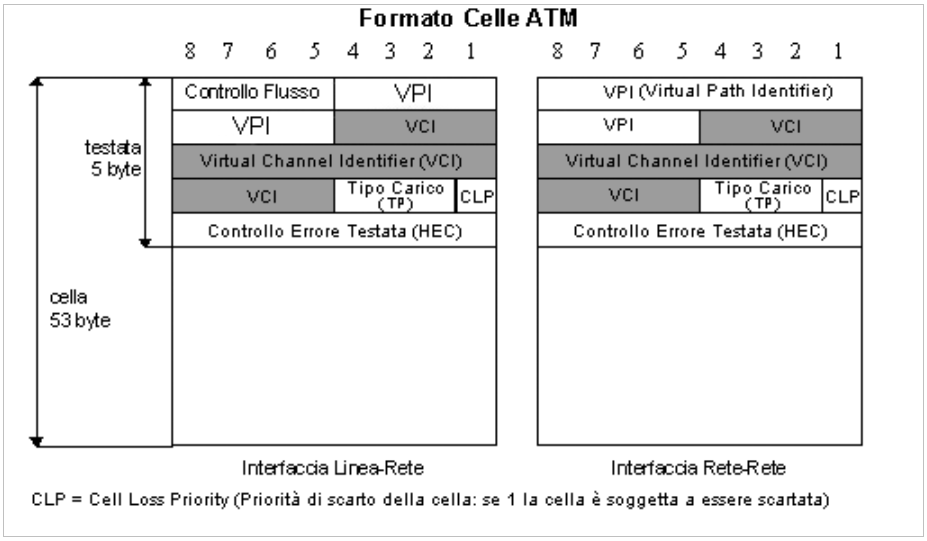
\includegraphics[scale=0.3]{images/ATM1.png}
    \caption{Formato di una cella ATM}\label{fig:1}
\end{figure}
\noindent
L'unità di trasmissione dei dati di ATM è detta cella, e ha una dimensione fissa di 53 byte, di cui 48 di 
payload (corpo di dati utili) e 5 di header. La lunghezza fissa e piccola della cella favorisce ritardi 
di elaborazione costanti e limitati durante la commutazione nei nodi nonché maggiori velocità di 
trasmissione estremamente vantaggiosi per il supporto alle varie tipologie di traffico.\\\\
ATM utilizza una tecnica di commutazione a circuito virtuale che lo rende appetibile per reti integrate 
nei servizi ad alta velocità di trasmissione: prima di inviare i dati si invia un pacchetto di handshake 
per configurare la connessione. Man mano che questo pacchetto attraversa gli switch ATM, questi calcolano 
l'instradamento, attribuiscono un identificatore (label) ai pacchetti di questa connessione e riservano 
risorse per la connessione stessa. A questo punto tutti i successivi pacchetti della connessione seguiranno 
lo stesso percorso com'è tipico della commutazione di circuito. Per il resto la trasmissione dei dati 
è segmentata in pacchetti di dimensioni fisse dette celle multiplate in maniera asincrona su canali logici 
o virtuali diversi per ciascuna connessione.\\\\
Le celle successive verranno identificate sulla base di un'etichetta. Quando una cella raggiunge uno switch, 
questo dovrà consultare una tabella indicizzata da porta in ingresso ed etichetta, ricavando la porta di 
uscita e la nuova etichetta da assegnare alla cella. Questa architettura molto semplice facilita 
l'instradamento in hardware permettendo di realizzare switch ad alta velocità (la commutazione 
per etichetta è più veloce rispetto alla commutazione IP basata sull'elaborazione in base a tabelle di 
routing indicizzate per sottoreti).
L'etichetta è composta di due valori presenti nell'header di ciascuna cella, VPI e VCI:\\
\begin{itemize}
    \item Il VPI (Virtual Path Identifier) identifica il path virtuale su cui il circuito virtuale è stato attivato.
    \item Il VCI (Virtual Channel Identifier) identifica il canale virtuale su cui il circuito virtuale è stato attivato.
\end{itemize}
\noindent
Gerarchicamente si ha che un circuito virtuale viene stabilito tramite il collegamento di più connessioni 
virtuali VC. Il VP è un canale virtuale gerarchicamente superiore al VC e infatti un VP può contenere 
fino a $2\textsuperscript{16}$ VC. Appositi dispositivi hardware, ad esempio switch ATM, sono in grado di gestire VP 
(con tutti i VC in essi contenuti) o anche direttamente i singoli VC.\\\\
Visto che tutti i pacchetti seguono la stessa strada, è garantita la consegna in ordine, ma non l'integrità 
informativa ovvero che tutti i pacchetti siano consegnati, perché sono sempre possibili code sugli switch 
e conseguenti perdite di pacchetti.\\\\
La velocità di trasmissione possibile va da 2 a 622 Mbps e anche oltre. È questa la velocità adatta alla 
tv ad alta definizione.\\\\
ATM consente inoltre di segmentare la banda sui diversi canali virtuali per suddividerla e offrirla ai 
diversi tipi di servizi di trasmissione tramite appunto l'uso dei VCC (VPI:VCI).\\\\
Per supportare vari tipi di traffico su ATM, e quindi vari tipi e livelli di qualità di servizio, 
sono stati definiti una varietà di modelli di servizio che si adattano sia al traffico telefonico 
(CBR: banda costante, forti garanzie su banda e ritardo) sia a quello IP (VBR: banda variabile, nessuna 
garanzia). A differenza delle reti IP, ATM deve dunque fornire una garanzia di trasporto, ovvero 
predeterminate prestazioni, per il particolare servizio utente richiesto.
\subsubsection{Applicazioni}
Sono possibili due modalità di implementazione di ATM su una rete di telecomunicazioni:\\
\begin{itemize}
    \item \textbf{LAN Emulation} (LANE): permette di far comunicare tra loro un insieme di terminali che 
    fanno parte di una stessa sottorete come appartenenti a una rete locale ATM senza utilizzare il 
    protocollo Ethernet con lo svantaggio però di dover creare connessioni ATM (cioè VC semipermanenti o 
    automatici). Di fatto la tal cosa non si è realizzata in favore invece delle comuni LAN Ethernet per 
    motivi di costo degli apparati ATM (switch ATM).
    \item \textbf{Classical IP su ATM} (CLIP): appresenta il modello che si è effettivamente affermato e 
    che consiste in uno schema di trasporto in cui router di interfaccia dialogano tra di loro attraverso 
    una rete ATM, che funge appunto da rete di trasporto, attraverso l'uso di circuiti virtuali permanenti 
    col vantaggio aggiunto di garantire QoS agli utenti e possibilità di VPN su scala geografica 
    (Ipsilon Networks).
\end{itemize}
\subsubsection{IP su ATM}
IP su ATM è stato introdotto all'inizio degli anni novanta per far fronte a esigenze di aumento del 
traffico che i router dell'epoca non erano in grado di soddisfare (gli switch ATM offrivano infatti 
prestazioni fino a 622 Mbit/s) e perché ATM offriva la possibilità di operare ingegneria del trafficoovvero 
pianificare/decidere come instradare il traffico all'interno della rete di trasporto grazie al meccanismo 
dei circuiti virtuali permanenti gestiti dinamicamente, ovvero modificabili a seconda del livello di 
congestione interno della rete.\\\\
Per trasportare traffico IP proveniente da una singola sorgente, si usa l'Adaptation Layer 5 (AAL5), 
che segmenta il pacchetto IP in celle. AAL5 prevede dunque la possibilità di segmentare pacchetti di 
dimensioni variabili fino a $2\textsuperscript{16}$ byte su un numero sufficiente di celle ATM con un overheadminimo. 
Ogni pacchetto AAL5 (CPCS-PDU) è coperto da un CRC per la rilevazione degli errori. Quindi, intendiamo 
per PDU l'insieme di celle ATM che trasportano questo pacchetto. Per ogni PDU, AAL5 ha un overhead di 8 
byte che si inserisce come trailer della PDU. Mentre un pacchetto AAL5 verrà trasmesso su più celle in 
AAL2, una cella potrà trasportare più pacchetti AAL2. Questa pratica comporta, però, un maggior carico 
di overhead sulla rete, dunque perdita di efficienza (Goodput).\\\\
Questa soluzione ha perso definitivamente i suoi vantaggi quando, con l'aumento delle prestazioni di 
elaborazione dei router IP fino al superamento delle capacità degli switch ATM, ATM ha mostrato tutti 
i suoi limiti in termini di gestione contemporanea di due diverse tipologie di rete (IP sopra e ATM 
sotto), nonché il problema del cablaggio che aumentava col quadrato dei terminali per le topologie 
a maglia completa adottate da ATM e quello intimamente connesso in termini di elaborazione, 
memorizzazione ed efficienza delle informazioni fornite dei protocolli di routing.\\\\
La nuova tecnologia di rete di trasporto che si è affermata è stata dunque IP over SDH/SONET e 
successivamente IP su MPLS su SDH/SONET.
\subsection{MPLS}
\subsubsection{Definizione}
Multiprotocol Label Switching (MPLS) è una tecnologia per reti IP che permette di instradare flussi di 
traffico multiprotocollo tra nodo di origine (Ingress Node) e nodo di destinazione (Egress Node) tramite 
l'utilizzo di identificativi (label) tra coppie di router adiacenti e semplici operazioni sulle etichette 
stesse. Le specifiche tecniche del protocollo sono state pubblicate dall'Internet Engineering Task 
Force nell'RFC 3031 e nell'RFC 3032.
\subsubsection{Introduzione}
MPLS è una tecnologia che prevede la determinazione di un percorso determinato per tutti i pacchetti 
di una comunicazione
\begin{itemize}
    \item il percorso viene identificato aggiungendo un’etichetta (Label) ad ogni pacchetto
    \item Questo meccanismo alleggerisce il lavoro dei router in quanto non devono più leggere le tabelle di 
    routing per stabilire il percorso di un determinato pacchetto
    \item Il nome multiprotocol deriva dal fatto che questa tecnologia lavora con IP, nonché con ATM e Frame Relay
    \item MPLS permette alla maggior parte dei pacchetti di essere inoltrati al livello 2 invece che al 3, 
    con notevoli guadagni di performance
\end{itemize}
\noindent
MPLS è una soluzione versatile per risolvere le problematiche delle reti moderne:
\begin{itemize}
    \item Velocità
    \item Scalabilità
    \item Gestione della qualità del servizio
    \item Ingegneria del traffico
    \item MPLS può essere implementato su reti ATM e frame relay esistenti
    \item I nuovi applicativi che sono stati sviluppati facendo capo alla tecnologia Internet richiedono 
    sempre più alle reti delle classi di servizio che ne garantiscano il funzionamento
    \item In questo ambito la tecnologia MPLS gioca un ruolo fondamentale
    \item MPLS ottimizza il routing e lo switching delle reti moderne
\end{itemize}
\subsubsection{Il Routing e lo Switching Tradizionale}
Internet è stato disegnato per applicativi abbastanza semplici: Trasferimento di files, login remoti, etc.
\begin{itemize}
    \item Per soddisfare questi bisogni bastava una piattaforma di routing software ed un hardware 
    che supporta connessioni T1/E1 o T3/E3.
    \item Attualmente si è diffuso lo switching di livello 3, una tecnologia che rende possibile 
    la commutazione dei sia a livello 2 che a livello 3 direttamente dall’hardware. Questa tecnologia 
    ha tolto il collo di bottiglia provocato dai router tradizionali.
    \item In ogni caso i pacchetti vengono instradati cercando sempre la strada migliore, questo senza 
    però tenere conto di parametri supplementari quali: i ritardi, la variazione del ritardo 
    (jitter / delay) e le congestioni delle reti.
\end{itemize}
\paragraph{Cos’è MPLS?}
\noindent
\\\\
MPLS è un framework specificato dal IETF (Internet Engineering Task Force) che prevede efficienza 
nel routing, switching di flussi di traffico che attraversano le reti. MPLS implementa le seguenti funzionalità:
\begin{itemize}
    \item Specifica i meccanismi per gestire i flussi di traffico tra hardware e software differenti.
    \item Rimane indipendente dai protocolli esistenti di Layer-2 e di Layer-3.
    \item Trova il modo di mappare gli indirizzi IP in „Label“ di lunghezza fissa, questi label vengono poi utilizzati 
    da tecnologie diverse di switching e routing per instradare i pacchetti.
    \item Interfaccia protocolli di routing e di riservazione delle risorse (RSVP) esistenti.
    \item Supporto di IP, ATM e frame-relay.
\end{itemize}
\paragraph{Come funziona:}
\noindent
\begin{enumerate}
    \item La rete costruisce automaticamente le tabelle di routing, i routers e gli switch IP+ATM del 
    “service provider” utilizzano dei protocolli di routing come OSPF, EIGRP, or IS-IS. Il “Label 
    Distribution Protocol” (LDP) utilizza la topologia di routing per stabilire i valori dei device 
    adiacenti. Questa operazione crea dei “Label Switched Paths”(LSPs) o mappe  preconfigurate tra le 
    diverse destinazioni. A differenza dei “permanent virtual circuits” (PVC), dove i VPIs/VCIs vengono 
    assegnati manualmente, i “labels” vengono assegnati automaticamente. 
    \item Un pacchetto arriva ad un “Edge Label Switch Router” (Edge LSR), il pacchetto viene processato 
    per determinare quale servizio Layer 3 necessita (QoS e bandwidth management). Basandosi sulle 
    decisioni di routing, il ”Edge LSR” seleziona ed applica un “label” al pacchetto, a questo punto 
    il pacchetto viene passato al prossimo LSR. 
    \item L’LSR nel core legge il “label” e lo rimpiazza con uno nuovo, come definito nella tabella. 
    Poi lo passa al prossimo LSR. Questa azione viene ripetuta per ogni LSR nel core.
    \item Il “Edge LSR” all’uscita toglie il “label”, legge l’header del pacchetto e lo passa 
    alla destinazione finale. 
\end{enumerate}
\subsubsection{IP + ATM}
MPLS consente agli switch ATM di comportarsi virtualmente come router IP. Questa proprietà è data dal fatto 
che il paradigma di “forwarding” usato da MPLS (label swapping) è esattamente lo stesso che viene 
implementato nell’hardware dagli switch ATM.\\\\
La differenza chiave tra uno switch ATM convenzionale ed uno switch ATM che supporta il “label switch” è 
nel software di controllo usato per stabilire i “virtual channel identifier” (VCI) delle tabelle dello 
switch. Uno switch ATM che supporta il “label switch” usa i protocolli di routing e il “Label Distribution 
Protocol” (LDP) per stabilire tali immissioni. 
\subsubsection{VPN basate su MPLS}
\begin{itemize}
    \item Si tratta di una peculiarità  di MPLS
    \item E’ possibile controllare il percorso di un pacchetto senza dichiarare esplicitamente tutti i 
    routers che lo compongono
    \item Creazione di tunnel nel percorso dei routers
\end{itemize}
\section{Metasploit}
\subsection{Penetration Test}
Il penetration test è il processo operativo di valutazione della sicurezza di un sistema o di una rete che 
simula l'attacco di un utente malintenzionato. L'analisi comprende più fasi ed ha come obiettivo evidenziare 
le debolezze della piattaforma fornendo il maggior numero di informazioni sulle vulnerabilità che ne hanno 
permesso l'accesso non autorizzato. L'analisi è condotta dal punto di vista di un potenziale attaccante e 
consiste nello sfruttamento delle vulnerabilità rilevate al fine di ottenere più informazioni possibili 
per accedere indebitamente al sistema. Il penetration test fornisce una stima chiara sulle capacità di 
difesa e del livello di penetrazione raggiunto nei confronti: 
\begin{itemize}
    \item delle vulnerabilità interne al sistema,
    \item delle vulnerabilità esterne al sistema,
    \item della sicurezza fisica.
\end{itemize}
\subsection{Procedura Black \& White Box}
I processi di penetration test possono essere effettuati in diverse modalità. La differenza consiste 
sulla quantità e qualità delle informazioni disponibili agli analisti riguardo ai sistemi analizzati.
\begin{itemize}
    \item \textbf{Black Box:} non presuppongono precedente conoscenza dell'infrastruttura oggetto di analisi 
    e gli esaminatori necessitano di determinare architettura e servizi dei sistemi prima di iniziare l'analisi.
    \item \textbf{White Box:} sono invece fornite conoscenze dettagliate dell'infrastruttura da esaminare, 
    spesso comprensive di schemi di rete, codice sorgente delle applicazioni e liste di indirizzi 
    IP presenti nella rete.
    \item \textbf{Grey Box:} sono varianti a queste metodologie.
\end{itemize}
\subsection{Analisi dell’architettura e rilevazione delle vulnerabilità}
Vengono acquisite inizialmente le informazioni principali sull'architettura della piattaforma e sui servizi 
offerti. Dall'analisi di questi dati deriva la scelta di come condurre il passo successivo, consistente in 
una enumerazione dei principali errori e problemi. 
\subsection{Attacco e redazione di un report}
L'attività si conclude nello sviluppo della reportistica composta dal report di analisi sommaria dedicato 
al management o executive summary, contenente l'analisi dell'impatto di rischio di quanto riscontrato e 
tempistiche per l'azione di rientro o mitigazione delle problematiche riscontrate, e dal report tecnico, 
contenente l'analisi dettagliata dei problemi e la soluzione tecnica. 
\subsection{Kali linux}
OS basato sulla distribuzione Debian GNU/Linux, permette di testare penetration testing OS, rewrite of 
BackTrack Linux e sviluppare sicurezza preventiva o offensiva. Ha più di 300 tool di supporto, è 
multilingua, è personalizzabile e flessibile, e ha una grande community per il supporto.
\subsubsection{Tool principali} 
\begin{itemize}
    \item Metasploit: security assesment framework
    \item NMAP: network scanner 
    \item John The Ripper \& Hashcat: password cracker
    \item Aircrack-ng: Wi-Fi crack
    \item Hydra: brute force attacks
    \item Maltego: information gathering
    \item Nikto: web scanner
    \item SET: Social Engineering Toolkit
    \item Bettercap: MITM attacks 
\end{itemize}
\subsection{Metasploit framework}
Si tratta di uno strumento open source per lo sviluppo e l'esecuzione di exploits ai danni di una macchina 
remota. È caratterizzato da: interfaccia a linea di comando, import da terze parti, exploitation manuale e 
azioni di forza bruta anch’esse condotte manualmente. Questa versione di Metasploit Project include anche 
Zenmap, un famoso port scanner, e un compilatore per Ruby, il linguaggio usato per questa versione. 
\begin{figure}[H]
    \center
    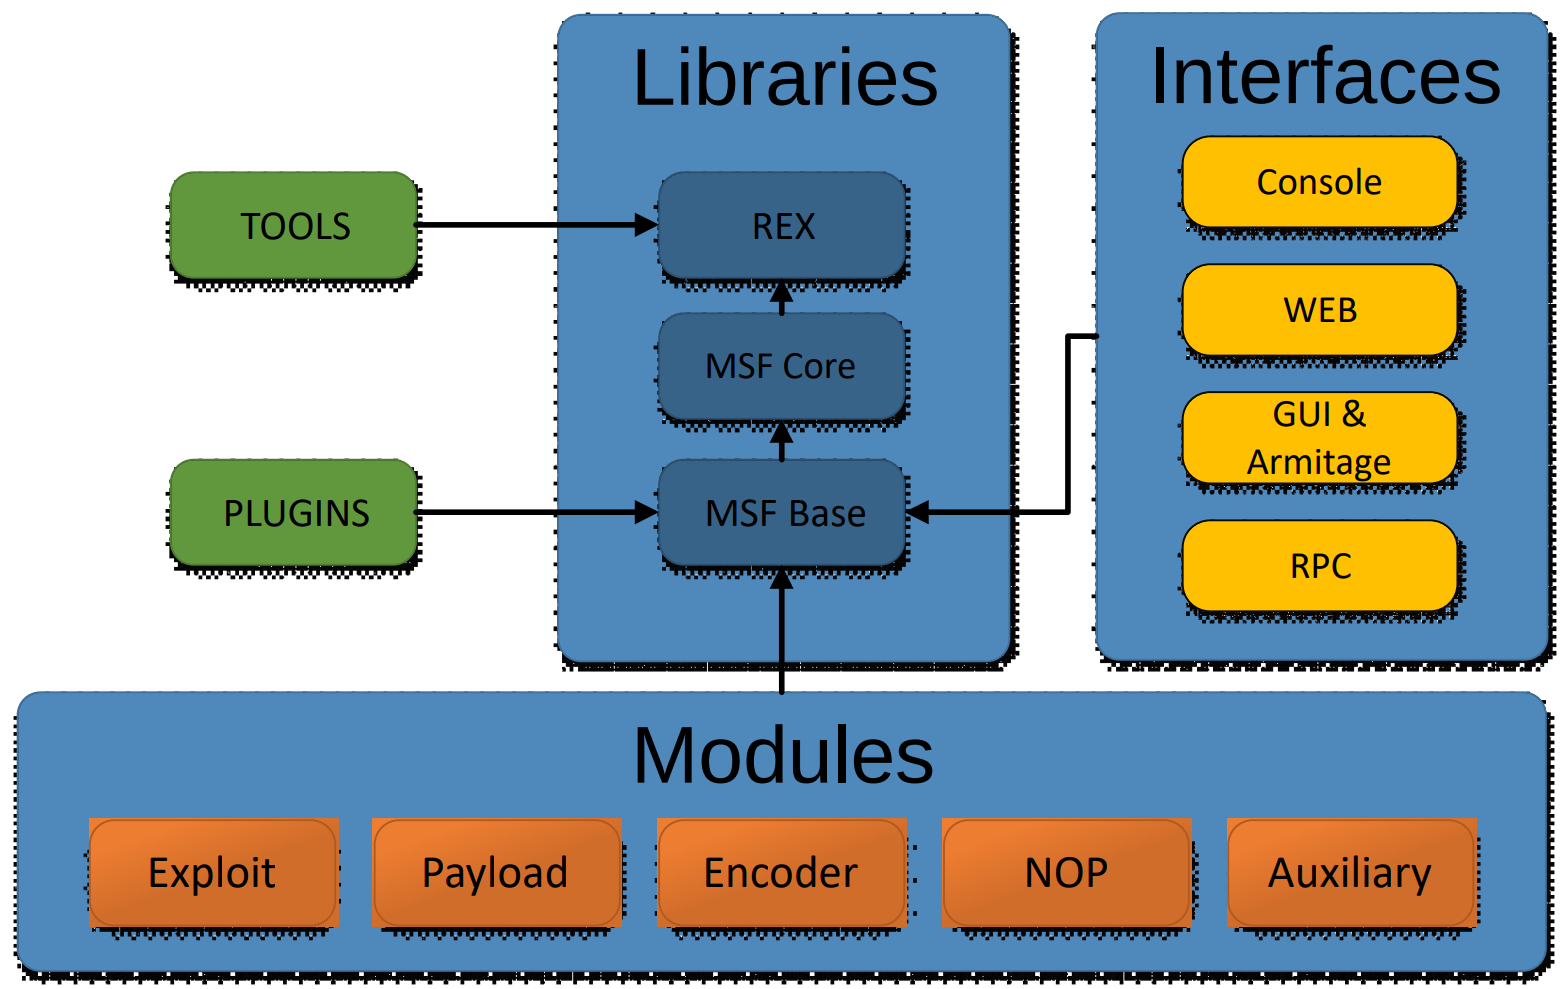
\includegraphics[scale=0.2]{images/SchemaMetasploit.png}
    \caption{Schema funzionale}\label{fig:1}
\end{figure}
\subsubsection{Definizione exploit}
Un exploit è una tipologia di script, virus, worm, porzione di dati o binario che sfrutta un bug 
o una vulnerabilità per creare comportamenti non previsti in software, hardware, o in sistemi elettronici, 
ad es. per ottenere l'accesso a sistemi informatici, permettere l'acquisizione dei privilegi amministrativi, 
o attacchi denial of service (DoS o il correlato DDoS). \\\\
\textbf{I passaggi fondamentali per l'exploiting di un sistema utilizzando Metasploit Framework comprendono:}
\begin{enumerate}
    \item Scegliere e configurare un \textbf{exploit} (codice che penetra in un sistema sfruttandone i bugs). 
    \item Controllare se il sistema attaccato è suscettibile all’exploit selezionato (facoltativo).
    \item Scegliere e configurare un \textbf{payload} (codice da eseguire sul sistema attaccato dopo esserci 
    penetrati con successo; per esempio una shell remota o un VNC server).
    \item Scegliere la tecnica di codifica in modo che l’intrusion prevention system (IPS) ignori il payload 
    codificato. 
    \item Eseguire l’exploit.
\end{enumerate}
\subsubsection{Metasploit Auxiliary Modules}
\begin{itemize}
    \item Exploit senza payload
    \item Scanning: tecnica per ricercare e mappare le debolezze di un'applicazione, di un computer o 
    di una rete
    \item Fuzzing: è una tecnica usata per individuare errori o falle di sicurezza del software. Il tester
     (o fuzz) invia al sistema dati casuali allo scopo di causarne il crash.
     \item Fingerprinting: generazione di una sequenza alfanumerica o stringa di bit di lunghezza prefissata 
     che identifica un certo file con le caratteristiche intrinseche stesse del file.
     \item Automated task
\end{itemize}
\subsubsection{Metasploit Encoders}
\begin{itemize}
    \item Code obfuscation
    \item Antivirus bypassing
    \item Encrypt payload (ShikataGaNai, Bloxor, Nonalpha)
\end{itemize}
\subsubsection{Metasploit Exploit \& Payload}
\begin{itemize}
    \item List of exploit
    \item Different OS: Unix, Windows, Linux, Android, Solaris, multi
    \item Payload (generate malware use exploit). \textbf{Stager:} connection attacker or victim. 
     \textbf{Stage:} malware.
\end{itemize}
\subsubsection{Console Commands}
\begin{itemize}
    \item msfconsole: apre la console di metasploit
    \item msfupdate: aggiorna il db degli exploit
    \item msfvenom: automaticamente genera il payload
    \item use: seleziona il modulo da usare
    \item set: assegna i parametri del modulo
    \item exploit: esegue l’attacco
\end{itemize}
\subsubsection{Come fare fuzz testing}
\begin{enumerate}
    \item Identificare i sistemi target
    \item Identificare input
    \item Generare informazione superflua
    \item Eseguire test usando informazione superflua
    \item Monitorare il comportamento di sistema
    \item Notificare i difetti
\end{enumerate}
\subsubsection{Tipi di bug detettati}
\begin{itemize}
    \item Problemi di asserzione e perdite di memoria questa metodologia è ampiamente utilizzata per 
    applicazioni di grandi dimensioni in cui i bug stanno compromettendo la sicurezza della memoria, 
    che è una grave vulnerabilità.
    \item Input non valido: i fuzzer vengono utilizzati per generare un input non valido che viene 
    utilizzato per testare le routine di gestione degli errori, e questo è importante per il software 
    che non ne controlla l'input. La semplice fuzzing può essere conosciuta come un modo per 
    automatizzare i test negativi.
    \item Correttezza dei bugs: Il fuzzing può anche essere usato per rilevare alcuni tipi di errori 
    di "correttezza". Come un database danneggiato, risultati di ricerca scadenti, ecc.
\end{itemize}
\section{Fibra ottica}

\section{Buffer overflow}
Il microprocessore è una tipologia particolare di circuito elettronico che si contraddistingue per 
essere interamente costituita da uno o più circuiti integrati di dimensioni molto ridotte. 
La tecnologia a microprocessore è attualmente quella più utilizzata per la realizzazione della CPU e 
della GPU (montate direttamente su una scheda madre, con la caratteristica di utilizzare, per tutte 
le sue elaborazioni, un insieme di istruzioni fondamentali di base (instruction set).\\\\
Si può trovare una lista di tutti i microprocessori della Intel, dal 4-bit Intel 4004 fino ai più 
moderni, al seguente link: \url{https://en.wikipedia.org/wiki/List_of_Intel_microprocessors}. \\
Per confrontarli invece si può andare su \url{https://en.wikipedia.org/wiki/Comparison_of_Intel_processors}.
\subsection{Intel i386}
Detto anche i80386, è una famiglia di microprocessori monolitici general purpose x86 dell'Intel Corporation 
prodotti tra il 1985 e il 2007. Le schede madri che supportavano i microprocessori Intel i386 erano 
molto complesse e costose, paragonate a quelle per i suoi predecessori, ma l'adozione su larga scala 
dei microprocessori Intel i386 ne favorì la diffusione. I microprocessori della famiglia Intel i386 
sono stati i primi microprocessori Intel dotati di architettura a 32 bit e modalità protetta con 
supporto hardware alla memoria virtuale paginata. Il successo e il basso costo di questi microprocessori 
permisero quindi la diffusione su personal computer dei primi sistemi operativi operanti in modalità 
protetta. L'Intel i386 fu anche la famiglia di microprocessori su cui nacque il kernel Linux.\\\\
Offre 16 registri di interesse al programmatore, i quali possono essere raggruppati nelle seguenti categorie:
\begin{figure}[H]
    \center
    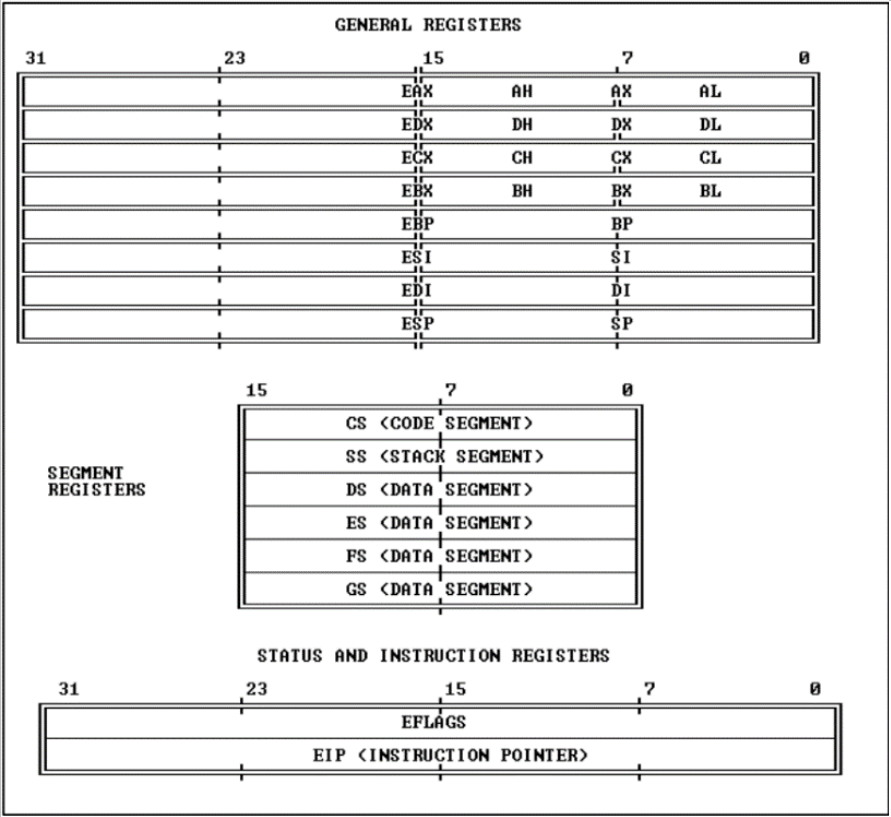
\includegraphics[scale=0.2]{images/BO1.png}
    \caption{Registri}\label{fig:1}
\end{figure}
\begin{itemize}
    \item Registri generali: 8 registri general purpose da 32-bit, usati principalmente per contenere 
    operandi per operazioni aritmetiche e logiche.
    \item Registri di segmento: registri special-purpose che determinano quale segmento di memoria è 
    indirizzabile e permettono ai designer di software di sistema di decidere tra un “modello piatto” 
    o lineare (singolo spazio contiguo) di organizzazione della memoria, oppure un modello segmentato.
    \item Registri di istruzioni e stato: registri special purpose usati per memorizzare e modificare 
    alcuni aspetti dello stato del processore 80386
\end{itemize}
\subsection{Tipi di buffer overflow}
\subsubsection{Buffer overflow della heap}
La memoria heap viene allocata in maniera dinamica dalle applicazioni run-time e solitamente contiene 
dati dei programmi utente. Gli heap overflow vengono solitamente usati dai cracker per abusare di 
programmi contenenti alcune vulnerabilità dovute ad insufficiente validazione degli input, calcolo 
sbagliato della memoria da allocare o superamento del limite massimo di memoria allocabile. 
L'attacco avviene come segue: se un'applicazione copia dei dati senza preventivamente controllare 
se trovano posto nella variabile di destinazione, il cracker può fornire al programma un insieme di 
dati troppo grande per essere gestito correttamente, andando così a sovrascrivere i metadati (cioè le 
informazioni di gestione) della heap, prossimi alla destinazione dell'insieme di dati. In questo modo, 
l'attaccante può sovrascrivere una locazione arbitraria di memoria, con una piccola quantità di dati. 
Nella maggior parte degli ambienti, questo può fornire all'attaccante il controllo dell'esecuzione del 
programma. 
\subsubsection{Buffer overflow dello stack}
lo stack è un’area di memoria in cui vengono salvate le variabili locali e i parametri passati alla funzione 
(gestito come LIFO). Qui i dati adiacenti al buffer che potrebbero essere sovrascritti dai dati extra sono 
il return address e il frame pointer. Se i dati in eccesso sovrascrivono frame pointer e return address, 
al termine dell’esecuzione la funzione tenterebbe di restituire il controllo all’istruzione puntata dal 
return address che potrebbe contenere:
\begin{itemize}
    \item L’indirizzo di un’area di memoria non accessibile: i dati in eccesso sono casuali, il programma 
    va in crash restituendo tipicamente un segmentation fault. È un esempio di come lo stack buffer 
    overflow possa essere utilizzato come attacco del tipo denial-of-service (DoS), compromettendo la 
    disponibilità del servizio colpito.
    \item Un indirizzo di memoria ben preciso: i dati in eccesso sono calcolati in modo da sovrascrivere 
    il return address con l’indirizzo di un’area di memoria a cui l’attaccante vuole avere accesso, o con 
    l’indirizzo in cui si trova il codice che l’attaccante vuole eseguire.
\end{itemize}
\begin{figure}[H]
    \center
    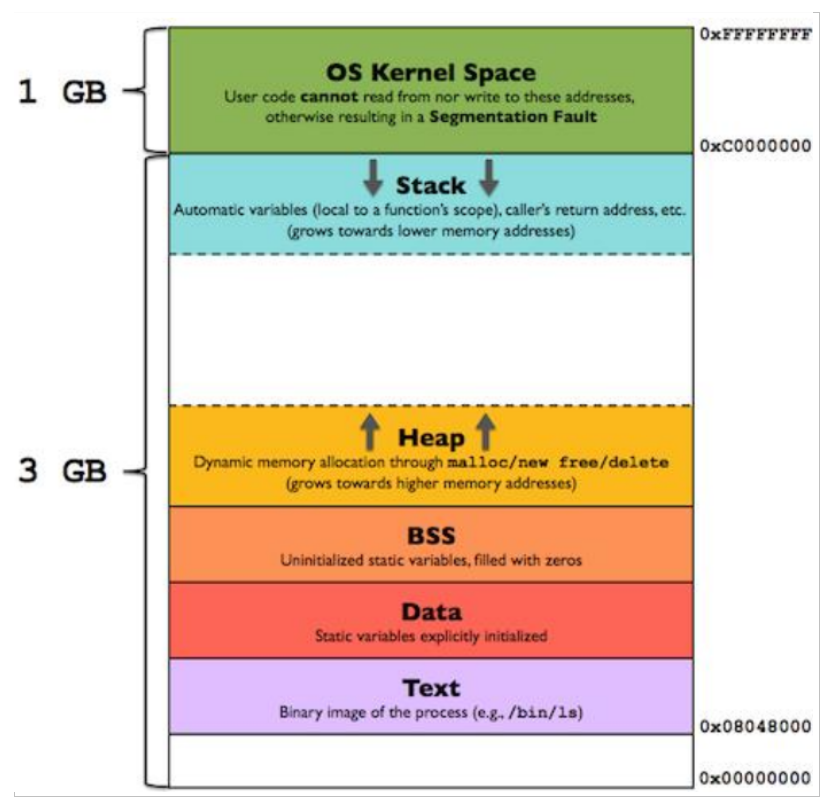
\includegraphics[scale=0.2]{images/BO2.png}
    \caption{Struttura della memoria}\label{fig:1}
\end{figure}
\subsubsection{Integer overflow}
Ovvero quando viene sorpassato il limite massimo per un Integer, che è 2dimensione in bit -1. 
Con len1 = len2 = 2147483648 = 231, l’operazione di somma len1 + len2 avrà quindi come risultato il 
valore 2147483648 + 2147483648 = 4294967296 = $2\textsuperscript{32}$. È proprio qui che si genera l’integer overflow. 
Il valore risultato della somma è troppo grande per essere memorizzato in una varabile di tipo int. 
Cosa succede quindi al programma? Il valore corretto viene troncato a 32 bit: nel nostro caso 4294967296 
diventa 0 che finisce col superare agevolmente il test dell’if e le due operazioni di memcpy vanno a 
sovrascrivere una zona di memoria superiore a quella allocata. In conclusione, alla funzione memcpy viene 
consentita la sovrascrittura dello stack ricadendo così nel più classico buffer overflow sullo stack del processo.
\begin{figure}[H]
    \center
    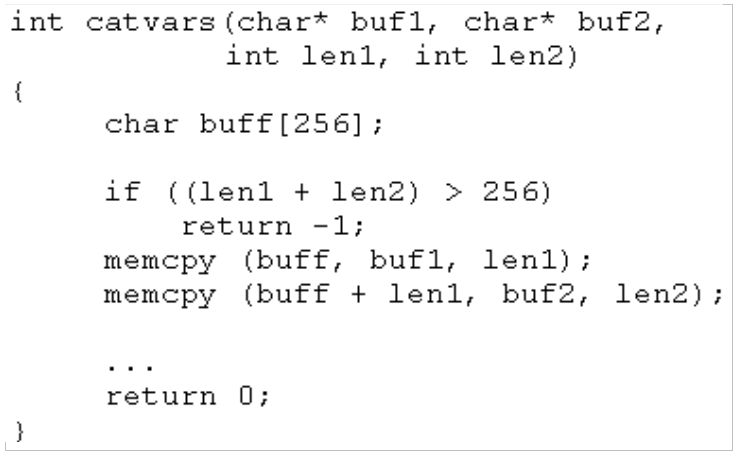
\includegraphics[scale=0.2]{images/BO3.png}
    \caption{Esempio di codice}\label{fig:1}
\end{figure}
\subsubsection{String format overflow}
Quando nei sistemi di print (ad es. in C) si usano delle formattazioni o ne vengono iniettate alcune maligne. 
Es. printf("\%s\%s\%s\%s\%s\%s\%s\%s\%s\%s\%s"); Ogni "\%s" cerca di visualizzare il contenuto di un buffer di 
caratteri dall'indirizzo iniziale presente sullo stack fino al carattere terminatore ("0"). Inserendo quindi molti 
“\%s", la funzione sposterà il puntatore in avanti fino ad aree di memoria non mappate nel frame dell'applicazione, 
così facendo cercherà di leggere da "indirizzi illegali", causando l'errore “segmentation fault” che manda in 
crash il programma.
\subsection{Stack pointer}
Ci sono 3 tipologie di puntatori alla memoria stack (la quale cresce verso il basso):
\begin{itemize}
    \item IP (Instruction Pointer): contiene l’indirizzo di ritorno.
    \item EBP (Base Pointer): è un registro che punta all’inizio dell’area dello stack utilizzata dalla 
    funzione corrente, in modo che nel caso di funzioni a cascata si possa sapere la posizione in memoria 
    delle variabili locali. Qui infatti parametri e variabili locali possono essere espressi in maniera 
    costante, secondo un offset fisso.
    \item ESP (Stack Pointer): indirizzo della richiesta dell’ultimo programma. Seguendo la logica della 
    pila LIFO, sarà il puntatore al top dello stack. 
\end{itemize}
\begin{figure}[H]
    \center
    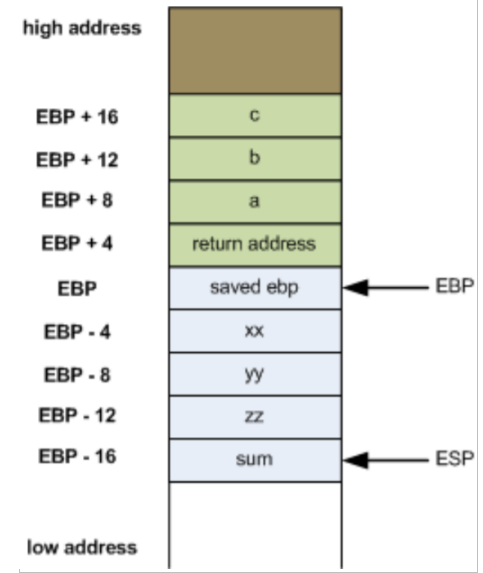
\includegraphics[scale=0.15]{images/BO4.png}
    \caption{Struttura dello Stack}\label{fig:1}
\end{figure}
Le operazioni sullo stack possono essere PUSH (inserisco l’elemento in cima alla pila) 
oppure POP (rimuovo il primo elemento della pila). 
\begin{figure}[H]
    \center
    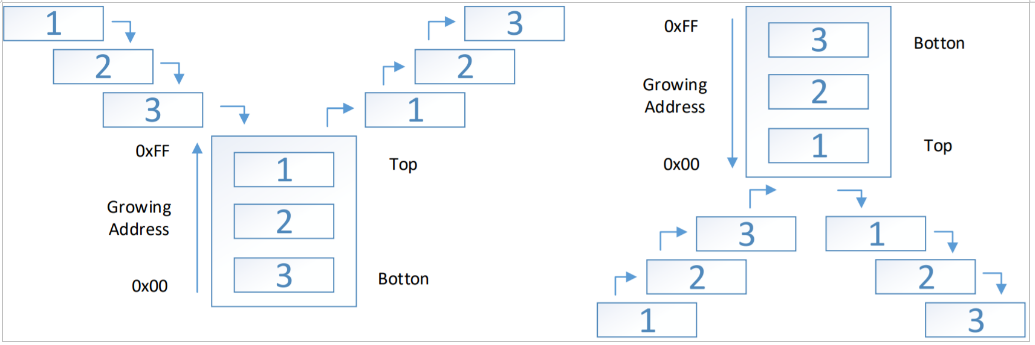
\includegraphics[scale=0.25]{images/BO5.png}
    \caption{Esempio operazioni sullo Stack}\label{fig:1}
\end{figure}
\subsection{Iniezione di shellcode}
Nel caso di un buffer overflow dello stack, spesso gli hacker ricorrono a iniezioni di shellcode nel buffer. 
L’overflow quindi non va ad inserire semplicemente istruzioni “extra” al buffer, bensì inserisce del codice 
eseguibile in linguaggio macchina (assembly) e la sovrascrittura del return address viene fatta in modo da 
rimandare al codice iniettato all’interno del buffer. Questo codice solitamente richiama una shell (con la 
chiamata alla funzione execve) che eseguirà con gli stessi privilegi del programma di partenza. 
\subsection{Protezione dello stack}
Per detettare gli overflow si può utilizzare StackGuard, il quale controlla il Canary Value o Canary Word. 
Questi non sono altro che un valore (solitamente posto prima del return address, StackShield) che, una volta 
sovrascritto da un buffer overflow, indica che è successo qualcosa che non va e quindi funge da controllo di 
sicurezza. Il programma “maligno” quindi terminerà la propria esecuzione a seguito di questo evento pericoloso. 
In linea di massima sono valori random che non sono prevedibili dall’attaccante e sono scelti a runtime. 
Esiste un tool che permette di vedere cosa sta succedendo all’interno di un programma in esecuzione o quello 
che è successo quando il programma in questione è crashato. Si può inoltre cambiare del codice nel programma 
per fare degli esperimenti di correzione di un bug o capire cosa sia successo. \\
\textbf{GNU Project Debugger (GDB):}
\begin{itemize}
    \item Run on program: gdb 'executable'
    \item Breakpoint: b funcion()
    \item Read address: x \$ebp, x \&variable
\end{itemize}
\section{Reverse Code Engineering}
\subsection{Motivazioni per il Reverse Code Engineering}
\noindent
\textbf{Hacking / Cracking:}
L'hacking è l'insieme dei metodi, delle tecniche e delle operazioni volte a conoscere, accedere e 
modificare un sistema informatico hardware o software, Con \textbf{cracking} si intende la modifica di un 
software per rimuovere la protezione dalla copia, oppure per ottenere accesso ad un'area altrimenti 
riservata. La distribuzione di software così reso privo di protezione è generalmente un'azione 
illegale a causa della violazione di un copyright. Il crack viene spesso ottenuto tramite il 
reverse engineering, tecnica che permette di capire la logica del software analizzando il suo 
funzionamento e le risposte a determinati input.\\\\
\textbf{Debugging:}
Un debugger in informatica è un programma/software specificatamente progettato per l'analisi e 
l'eliminazione dei bug (debugging), ovvero errori di programmazione interni al codice di altri programmi.\\\\
\textbf{Software (Malware) analysis:}
L'analisi dei malware consiste nello studio delle funzionalità, dell'origine e dell'impatto di un dato 
campione di malware, come virus, worm, trojan, rootkit o backdoor. Per malware o software dannoso si 
intende qualsiasi software destinato a danneggiare il sistema operativo host o per rubare dati 
sensibili da utenti, organizzazioni o società. Il malware può includere software che raccoglie 
informazioni utente senza autorizzazione.
\subsection{Approccio di reverse code engineering}
\begin{figure}[H]
    \center
    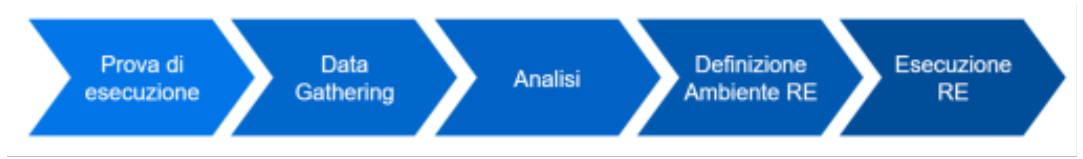
\includegraphics[scale=0.3]{images/Macrofasi.png}
    \caption{le 5 macrofasi}\label{fig:1}
\end{figure}
\subsubsection{Prova di esecuzione}
La prova di esecuzione ci può fornire numerose informazioni:
Ci permette di studiare il comportamento del programma e le connessioni verso eventuali servizi 
(server) esterni, ci permette di capire come funziona il meccanismo di protezione del software 
(gestione password, controllo numero di serie e/o licenza) e infine di raccogliere informazioni 
generali sul software e sull’ambiente di deployment di quest’ultimo.\\\\
Nel caso l’eseguibile si tratti di un malware è necessario fare questo procedimento in un 
ambiente isolato. 
\subsubsection{Data Gathering}
In questa fase è possibile raccogliere altre informazioni sull’eseguibile:
Si utilizzano software per la Detection di ambienti di sviluppo e versioni.
Vengono raccolti dati sul linguaggio di programmazione, sulla protezione e sul 
sistema operativo utilizzato. Il Data Gathering è una attività necessaria per le fasi successive.
\begin{figure}[H]
    \center
    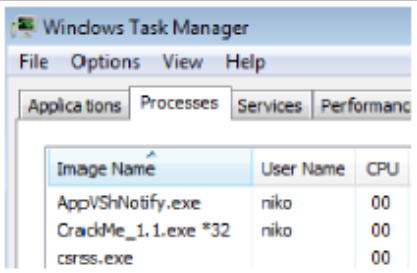
\includegraphics[scale=0.3]{images/RCE1.png}
    \caption{Esempio}\label{fig:1}
\end{figure}
\noindent
Informazioni raccolte: MS Windows, Applicazione a 32 bit, Dephi,non pacchetizzato.
\subsubsection{Analisi}
Faccio un’analisi dettagliata del software e decido la tipologia di approccio che voglio prendere.
Inoltre in questa fase viene definito l’obiettivo finale.
Esempio:\\\\
\begin{itemize}
    \item Obiettivo? Messaggio positivo
    \item Tipologia di approccio? Patch del file
    \item Protezione? Nessuna
\end{itemize}
\subsection{Definizione dell’ambiente per RCE}
In questa fase scegliamo, in base all’obiettivo prefissato precedentemente, l’ambiente di analisi 
che andremo ad utilizzare. Gli ambienti di analisi conosciuti sono i seguenti:
\begin{itemize}
    \item \textbf{Virtual machine:} software che, attraverso un processo di virtualizzazione, 
    crea un ambiente virtuale che emula tipicamente il comportamento di una macchina fisica 
    (PC client o server) grazie all'assegnazione di risorse hardware (porzioni di disco rigido, 
    RAM e risorse di processamento) ed in cui alcune applicazioni possono essere eseguite come 
    se interagissero con tale macchina. Tra le più conosciute abbiamo: VMware server, 
    VMware workstation, VMware player, XEN, QEMU, KVM.
    \item \textbf{Sandbox:} Una sandbox è un meccanismo che permette di eseguire dei file all’interno 
    di un ambiente ristretto, solitamente vengono utilizzate per testare applicazioni non attendibili 
    o potenzialmente dannose.
    Fornisce un set di risorse ristretto al programma che deve essere testato, come ad esempio un’area 
    ristretta di memoria o un insieme di chiamate di sistema limitate.
    Solitamente gli viene tolta la possibilità di connettersi alla rete e di interfacciarsi con il 
    sistema ospite.
    Le sandbox possono essere viste come una sorta di virtualizzazione, con la differenza che 
    all’interno di una macchina virtuale in cui vogliamo testare un virus viene virtualizzato un 
    intero sistema operativo mentre nelle sandbox solamente la struttura che permette di eseguire il programma.
    \item \textbf{Esecuzione su macchina fisica:} L’eseguibile viene fatto girare su un sistema nativo.
    \item \textbf{Viene utilizzato un software di analisi:} Si utilizza un software che consente l’analisi del 
    codice dell’eseguibile, come ad esempio un Disassembler che permette di ricostruire il codice assembly del 
    file, un Decompiler  che consente di ricostruire il codice sorgente (a grandilinee) o un debugger che 
    consente l’esecuzione graduale del software.
\end{itemize}
\subsection{Esecuzione RE}
Svlogiamo i seguenti passi:
\begin{itemize}
    \item Inizio del lavoro sul programma compilato
    \item Definizione degli obiettivi
    \item Ricerca della strada per arrivare alla soluzione
    \item Persecuzione dell’obiettivo
\end{itemize}
\textbf{Esempio:} Inizio del lavoro sul programma compilato: Estrattore Strada per arrivare alla 
soluzione: usiamo un disassembler (processori 32 bit, processori 64 bit, alri sistemi) Persecuzione 
dell’obiettivo:
\begin{figure}[H]
    \center
    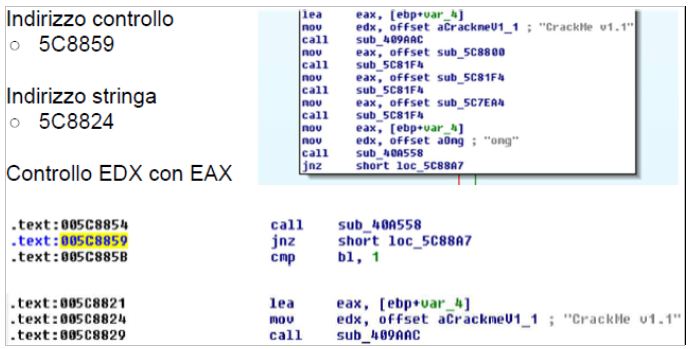
\includegraphics[scale=0.3]{images/RCE2.png}
    \caption{Esempio}\label{fig:1}
\end{figure}
\subsection{Programmi più utilizzati per l’RCE}
\noindent
\textbf{OllyDbg:} OllyDbg è un debugger, disponibile solo in versione a 32 bit, per sistemi Microsoft Windows. 
OllyDbg traccia i registri, riconosce le funzioni e i parametri passati alle principali librerie standard, 
le chiamate alle API del sistema operativo, eventuali salti condizionali, tabelle, costanti, variabili e 
stringhe. Tutto questo, sia all'interno di DLL, che di eseguibili EXE.\\\\
\textbf{X64Dbg:} Un debugger open source binario per Windows, finalizzato all'analisi dei malware e al 
reverse code engineering di file eseguibili. Ci sono molte funzioni disponibili e un sistema di plugin 
completo per aggiungere funzionalità.\\\\
\textbf{IDA Pro:} L'Interactive Disassembler, più comunemente conosciuto con il nome IDA, è un 
disassembler largamente usato per il reverse engineering. Supporta numerosi formati di file eseguibili 
per diversi processori e sistemi operativi.
Sebbene IDA effettui una grande quantità di reverse engineering in automatico, ottenendo informazioni 
sui riferimenti incrociati (cross-references o XREFs) tra le varie sezioni, sui parametri delle chiamate 
API, e altro, è comunque caratterizzato soprattutto dall'interattività. Un tipico utente di IDA inizierà 
con un listato generato automaticamente per poi rinominare, commentare, o aggiungere in altri modi 
informazioni al disassemblato, finché diventa chiaro cosa fa, rendendo IDA un ottimo strumento per il 
reverse engineering.\\\\
\textbf{Ghidra:} Ghidra è uno strumento per il reverse code engineering gratuito e open source sviluppato 
dalla National Security Agency (NSA). Ghidra è visto da molti ricercatori come un concorrente di IDA Pro 
e JEB Decompiler. Il software è scritto in Java usando il framework Swing per la GUI. Il componente 
Decompiler è scritto in C++. 
\subsection{Reverse Code Engineering in ambiente Android}
E’ possibile utilizzare un Android virtual machine chiamata Dalvik, l’estensione dei file è .apk.
Un file .apk ha la seguente struttura:
\begin{itemize}
    \item AndroidManifest.xml (package name, version, permissions, \dots)
    \item Classes.dex (Android bytecode)
    \item Res/ (Resources files)
    \item Lib/ (libs)
    \item META-INF (signatures)
\end{itemize}
\begin{figure}[H]
    \center
    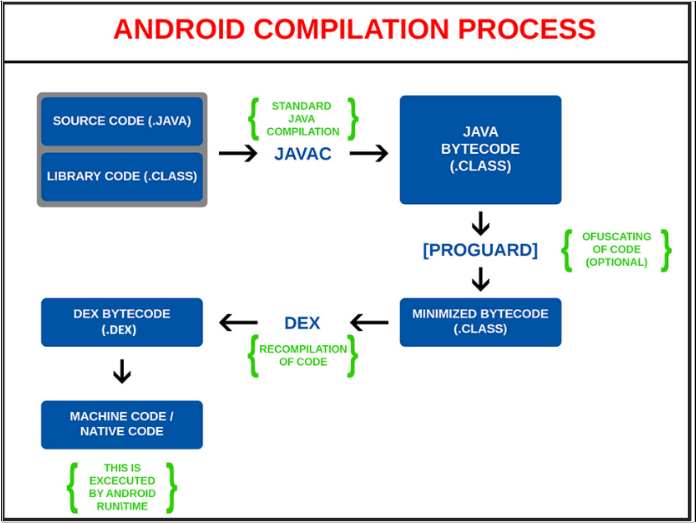
\includegraphics[scale=0.27]{images/RCE3.png}
    \caption{Schema del processo di compilazione}\label{fig:1}
\end{figure}
\begin{figure}[H]
    \center
    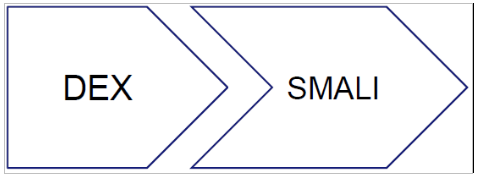
\includegraphics[scale=0.3]{images/RCE4.png}
    \caption{Processo di Disassembling}\label{fig:1}
\end{figure}
\noindent
\textbf{.dex} (Dalvik Executable): file compilato, Android byte code.\\
\textbf{.smali}: Codice disassemblato, più leggibile per l’uomo. \\\\
\textbf{Apktool:} Uno strumento per il reverse engineering per le applicazioni Android. Può ricostruire 
le risorse in forma quasi originale, in seguito è anche possibile modificare il codice. È Multi piattaforma.
\subsubsection{Smali}
\noindent
\textbf{Tipi in Smali:} V \(void\), Z \(boolean\), B \(byte\), S \(short\), C \(char\), F \(float\), 
I \(int\), J \(long\), D \(double\), parentesi quadrata \(array\).\\
\textbf{Sintassi Classi in Smali:} Nome del package separato da ‘/’, L \(prefisso\), ; \(suffisso\)\\
Esempio: \(Lcom/example/myapp/MyClass\)
\begin{figure}[H]
    \center
    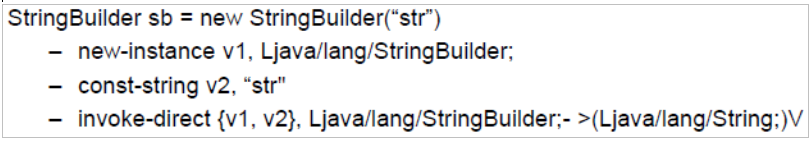
\includegraphics[scale=0.4]{images/RCE5.png}
    \caption{Java vs Smali}\label{fig:1}
\end{figure}
\begin{figure}[H]
    \center
    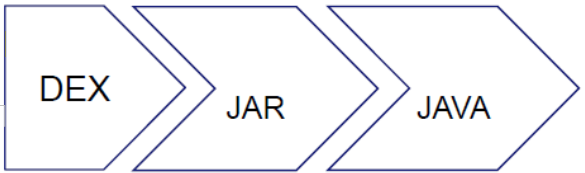
\includegraphics[scale=0.3]{images/RCE6.png}
    \caption{Java Decompiler}\label{fig:1}
\end{figure}
\noindent
\textbf{JD-GUI:} è un Decompilatore Java che prende in input un .jar e restituisce in output un .java\\
\textbf{Dex2jar:} Converte un file DEX (Conver Dalvik bytecode) in file JAR (java bytecode).
\subsection{Approccio generale per RCE su Android}
\begin{itemize}
    \item Unzip APK e disassemblamento classes.dex
    \item Analisi statica del codice
    \item Injection del byte-code nell’app
    \item Riassemblamento class.dex \& zip/firma dell’APK
\end{itemize}
\begin{figure}[H]
    \center
    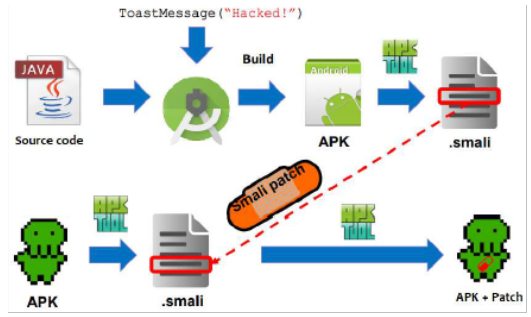
\includegraphics[scale=0.5]{images/RCE7.png}
    \caption{Schema riassuntivo dell'approccio}\label{fig:1}
\end{figure}
\section{Honeypot e Honeynet}
\subsection{Teoria}
\subsubsection{Cos'è un honypot}
\noindent
\begin{quotation}\small\selectlanguage{italian}
“A honeypot is an infomation system resource whose value lies in unauthorized or illicit use of that resource.” 
- Lance Spitzner    
\end{quotation}
E’ un sistema hardware o software usato come “esca” per i pirati informatici, portando benefici 
in termini di protezione. E’ un \textbf{finto sistema vulnerabile} che ne simula uno vero. Consiste generalmente 
in un computer (spesso virtualizzato) o ad un sito volutamente esposto di cui si vuol far credere sia 
un contenitore di informazioni preziosi, ma che in realtà è \textbf{ben isolato} e contiene \textbf{informazioni fittizie} 
che simulano i dati relativi all’azienda. Potrebbe essere un file, un record o un indirizzo IP non utilizzato.
Produce un \textbf{log} che memorizza le azioni svolte dall’attacker.
\subsubsection{Vantaggi}
\noindent
\textbf{Registra le azioni} del mal intenzionato. Insieme ad un sistema di IDS (più precisamente un Anomaly 
Detection System) permette di dare continuità all’azione dell’hacker raccogliendo maggiori informazioni 
tali da poter conoscere meglio il proprio nemico. Fa perdere tempo all’hacker. Isolando un virus 
l’azienda ne può studiare il comportamento e un sistema di contromisura da adottare. 
Creare statistiche dell tipologie di malware, virus o worm ricevuti
\subsubsection{Svantaggi}
Gli honeypot possono portare rischi alla rete, devono essere quindi gestiti e utilizzati con cura. 
Se non sono ben protetti l’attacker potrebbe usarli per entrare in altri sistemi (per esempio se l’honeypot fosse in LAN).
Incrementa il traffico di rete.
E’ presente una lista nel deep web dove sono presenti tutti gli honeypot conosciuti nel mondo.
\subsubsection{Tipi di Honeypot}
\noindent
Soliamente sono classificati in base alla modalità di interazione con l’utente.
\begin{itemize}
    \item Honeypot puriSfruttare un web server o un sito esposto come honeypot. Creare un file adminLogin.php (nome che attira):
    \item Honeypot ad alta interazione 
    \item Honeypot a bassa interazione
    \item Honeynet/honeyfarm
\end{itemize}
\paragraph{Honeypot puri}
\noindent
\\
Sono macchine fisiche presenti in una rete di produzione in cui è possibile accederci in remoto per monitorare gli attacchi. 
Non è il metodo migliore per implementare un honeypot.
\paragraph{Honeypot ad alta interazione}
\noindent
\\
In un computer fisico vengono virtualizzate più macchine. Permettono di simulare in modo fedele l’ecosistema di produzione 
aziendale fornendo all’hacker il modo di poter utilizzare una varietà di servizi reali con lo scopo di far perdere del tempo.
Pro: forniscono recupero veloce della macchina in caso di manomissione (perché virtuale). In genere offrono un miglior 
servizio di sicurezza essendo difficili da rilevare. Contro: costi di manutenzione elevati.
\paragraph{Honeypot a bassa interazione}
\noindent
\\
Solitamente emulano specifici servizi di rete. Sono software che emulano sistemi operativi e servizi più utilizzati 
dagli attaccanti per portare avanti un attacco. Pro: facili da installare e sicuri. Contro: catturano una quantità 
inferiore di informazioni. Honeyd = vengono virtualizzati una serie di computer configurati per simulare diversi 
tipi di server.
\paragraph{Honeynet/Honeyfarm}
\noindent
\\
E’ un insieme di honeypot. Il bisogno di mettere in relazione più honeypot è legato al fatto che un singolo honeypot può non 
essere sufficiente a ricoprire una rete molto ampia e diversificata. Una honeyfarm è una raccolta centralizzata di honeypot 
e strumenti di analisi.
\subsubsection{Famiglie di honeypots}
\paragraph{Database honeypots}
\noindent
\\
I database spesso vengono attaccati tramite SQL Injection. Alcuni firewall forniscono/supportano l’architettura honeypot in 
modo tale da spostare gli intrusi su un database trappola mentre l’applicazione web rimane funzionante.
\paragraph{Web honeypots}
\noindent
\\
Sfruttare un web server o un sito esposto come honeypot. Creare un file adminLogin.php (nome che attira): \\
\begin{lstlisting}[language=java, basicstyle=\small]
function sendData()
{
    $socket = 
    stream_socket_client("tcp://127.0.0.1:60099", $errno, $errorMessage);
    stream_set_timeout($socket, 1, 0);
    socket_set_blocking($socket, 1);
    if ($socket === false) {
        return FALSE;
    }
    $dataToSend = json_encode(array(
        'server' => $_SERVER,
        'post' => $_POST,
        'get' => $_GET,
        'file' => __FILE__,
        'pid' => getmypid(),
        'uid' => getmyuid()
    ));
    while (strlen($dataToSend)!==0)
    {
        $bytesWritten = fwrite($socket, $dataToSend);
        $dataToSend = substr($dataToSend, $bytesWritten);
    }
    fclose($socket);
    return TRUE;
}
\end{lstlisting}
\begin{lstlisting}[language=html, basicstyle=\small]
<html>
    <head>
        <title>BitNinja Honeypot</title>
    </head>
    <body>
        This is a honeypot file. Please leave it.
    </body>
</html>
\end{lstlisting}
\begin{lstlisting}[language=php, basicstyle=\small]
<?php
    /*
     * Finaly, we flush the output - send the content to the client - and
     * call the sendData() function to send the request to BitNinja.
     */
     flush();
     sendData();
?>
\end{lstlisting}
\paragraph{Service honeypots}
\noindent
\\
E’ un’applicazione che inoltra il traffico in ingresso dalla porta 22 (SSH) al serrver HaaS, dove Cowrie honeypot 
simula un dispositivo e registra i comandi eseguiti. Il computer rimane in uno stato sicuro perché tutto il traffico 
è rediretto al server.
\begin{figure}[H]
    \center
    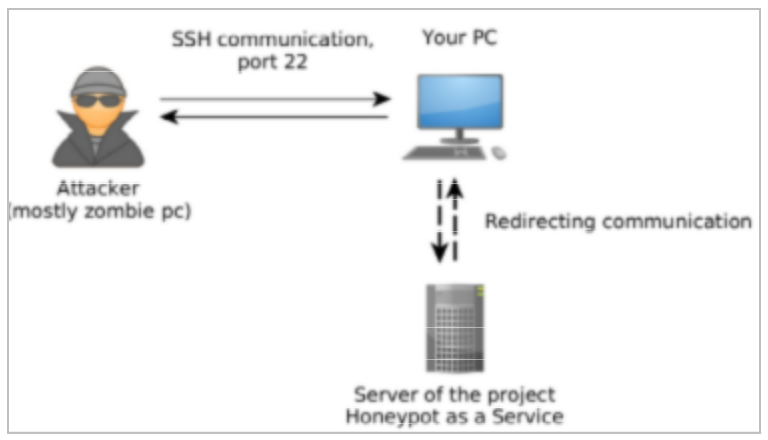
\includegraphics[scale=0.3]{images/HP1.png}
    \caption{Schema riassuntivo}\label{fig:1}
\end{figure}
\paragraph{Spamtrap honeypots}
\noindent
\\
Si tratta di indirizzi e-mail pubblicati da alcune aziende di soluzione anti-spam o da singoli individui su diversi 
siti e/o forum web. Nessuno utilizza questi indirizzi per inviare mail, quindi se si dovesse ricevere un messaggio 
da questo indirizzo vuol dire che qualcuno sta cercando di spammare.\\\\
Gli spammer abusano spesso di risorse come server di posta open mail relay e gli open proxy per effettuare attività di spam.
Questi honeypot possono mostrare l’indirizzo IP degli spammer e permettono di fermare in massa un’azione di spam. 
E’ possibile ricavare anche l’indirizzo mail dello spammer perché tipicamente per assicurarsi che il sistema sia funzionante 
invia mail a se stesso come prima fase di test.
\paragraph{SCADA honeypots}
\noindent
\\
Supervisor Control And Data Acquisition è un sistema di software e hardware che permette ad un’organizzazione industriale di:
Controllare i processi di industria localmente o in remoto. Interagire direttamente con sensori, valvole, motori tramite HMI 
(Human-Machine Interface).Registrare eventi in un log file. Un honeypot che simula il comportamento di un sistema SCADA è a 
bassa interazione che modifica l’indirizzo MAC dei suoi adattatori in modo che gli aggressori non possano facilmente “imprimerlo”.
Simula molto bene il comportamento di un sistema industriale rallentando le risposte per rendere uguale la velocità di risposta 
di un sistema ad alto carico come uno industriale. Come implementare uno SCADA honeypot:
\begin{itemize}
    \item Installare le librerie e dipendenze necessarie: 
    \begin{lstlisting}[language=bash, basicstyle=\small]
    sudo apt-get install libsmi2ldbl snmp-mibs-downloader python-dev 
    llibevent-dev libxslt1-dev libxml2-dev
    \end{lstlisting}
    \item Installare python
    \begin{lstlisting}[language=bash, basicstyle=\small]
    sudo apt-get install python-pip
    \end{lstlisting}
    \item Installare MySQL e le dipendenze
    \begin{lstlisting}[language=bash, basicstyle=\small]
    sudo apt-get install python-dev libmysqlclient-dev
    sudo apt-get install MySQL-python
    \end{lstlisting}
    \item Installare Conpot
    \begin{lstlisting}[language=bash, basicstyle=\small]
    sudo pip install conpot
    \end{lstlisting}
    \item Run Conpot
    \begin{lstlisting}[language=bash, basicstyle=\small]
    sudo conpot -template default
    \end{lstlisting}
\end{itemize}
\subsection{Pratica}
\subsubsection{Implementazioni di honeypots}
\textbf{Conpot:} è un sistema di controllo lato server di bassa interazione facile da testare e deployare.\\
\textbf{Cowrie:} è un sistema progettato per catturare connessioni SSH e Telnet. Registrazione delle informazioni 
sulla sessione. Questi tipi di honeypot sono spesso connessi a Internet per monitorare gli strumenti, gli script e 
gli host utilizzati dagli autori di attacchi di password.\\
\textbf{Dionaea:} è honeypot lato server a bassa interazione che emula un systema o device vulnerabile. 
L’obiettivo è avere una copia del malware per poterne studiare il comportamento. Esso supporta diversi 
protocolli a livello rete e applicativo tra cui SMB, http, FTP, TFTP MySQL, SIP (VoIP). Ultimamente ha 
sviluppato supporti per emulare un dispositivo IoT, smartTV o XBOX con protocolli UpnP e MQTT.\\
\textbf{Glastopf:} è un emulatore di web server scritto in python. Le informazioni raccolte riguardano attacchi 
SQLInjection, file inclusion attack (script presenti in pagine web) \dots \\
\textbf{Kippo:} è un honeypot di SSH di media interazione scritto in Python. Registrainformazioni riguardanti 
attacchi di brute force e l’intera interazione di shell eseguita dall’attacker. E’ sotto licenza BSD. 
Viene utilizzato il suo sucessore Cowrie (migliore rispetto a Kippo).
\subsubsection{Dove mettere un honeypots}
\paragraph{LAN}
\noindent
\\
\textbf{Vantaggi:} Cattura attacchi interni alla rete. Riesce anche a detettare mal configurazioni del firewall \\
\textbf{Svantaggi:} L’attacco può contaminare anche le macchine presenti all’interno della rete perché bisogna 
esporre all’esterno l’honeypot 
\paragraph{DMZ}
\noindent
\\
\textbf{Vantaggi:} Intrappola attacchi al servizio pubblico dell’azienda.\\
\textbf{Svantaggi:} Non è possibile intrappolare attacchi interessanti (perché in genere una DMZ non è pienamente accessibile 
\paragraph{Rete separata}
\noindent
\\
\textbf{Vantaggi:} Non incrementa il rischio per la rete interna. Riduce il traffico d’attacco al firewall\\
\textbf{Svantaggi:} Non intrappola attacchi interni. Riduce gli allarmi prodotti dal firewall (fa un po come 
da scudo assorbendo gli attacchi)
\subsubsection{LOG di un honeypot}
\begin{figure}[H]
    \center
    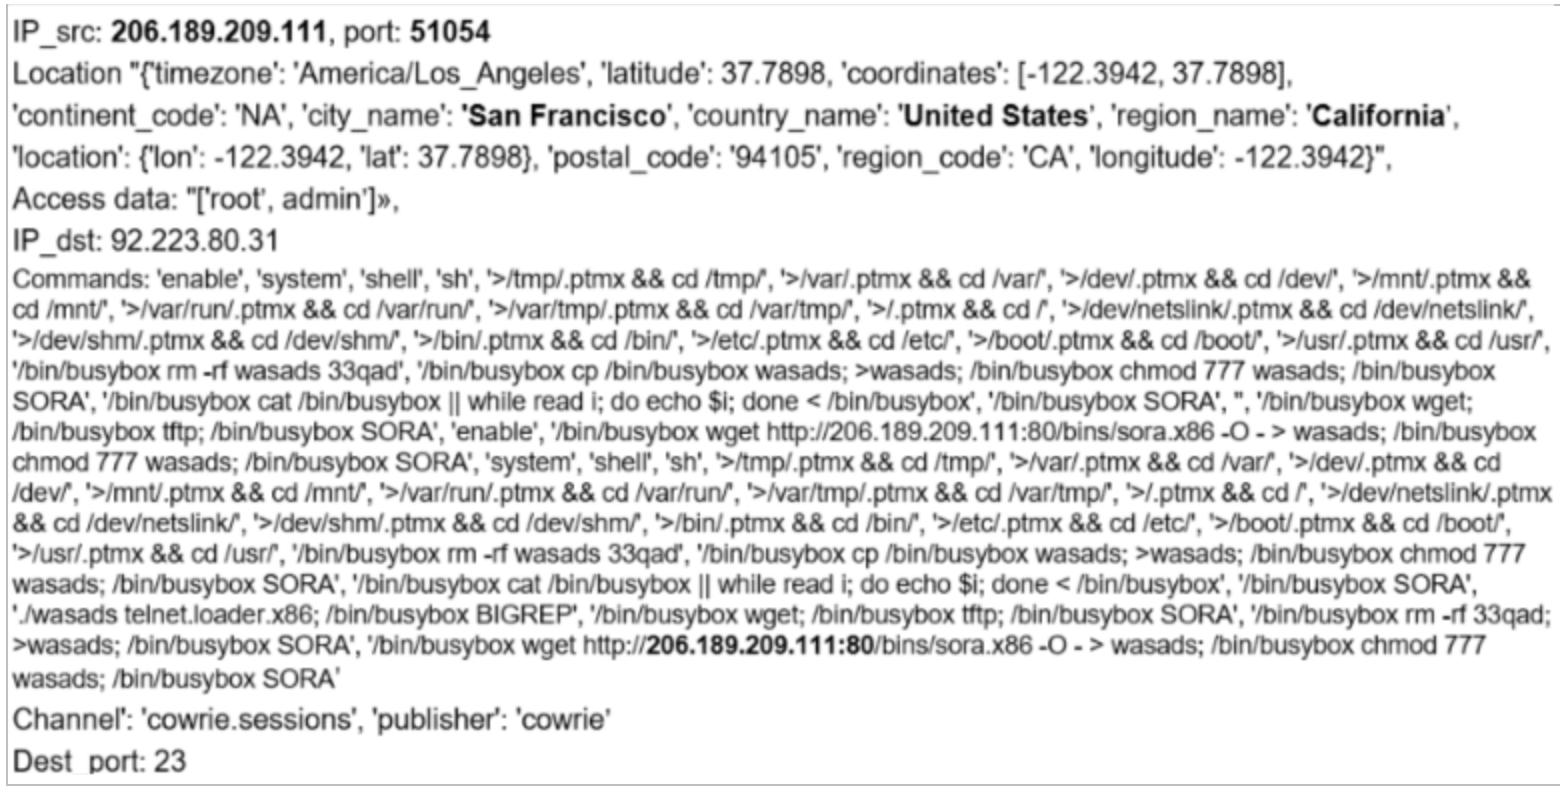
\includegraphics[scale=0.25]{images/HP2.png}
    \caption{Esempio di un LOG}\label{fig:1}
\end{figure}
\textbf{IP-src} = ip dell'hacker con relativa location \\
\textbf{IP-dst} = honeypot\\
\textbf{Commands} = comandi eseguiti dall’hacker. Alla fine è possibile notare un wget con il relativo IP.  
è possibile capire che l’attacker vuole scaricare un virus che risiede nella sua macchina. Facendo così la scarica nella macchina infettata.\\
\textbf{Dest-port} = porta di  uscita del log \\
\subsubsection{Come “detettare” un honeypot}
Log overflow: si possono fare azioni non malevole per intasare il log file
Se l’attacco è più facile del dovuto allora molto probabilmente c’è un honeypot di mezzo.Come è possibile notare non è presente un metodo 
vero e proprio perché un honeypot è un vero o proprio servizio/dispositivo. 
\subsubsection{Come esportare un log file}
Se l’honeypot è una macchina virtuale utilizzare una seconda NIC connessa alla rete di management. Il ciò deve implicare che l’attacker 
non deve avere il modo di poter vedere le connessioni aperte sulla macchina. Dall’interfaccia di management è possibile accederci in remoto.
\section{Darknet, Traffic Analysis and Botnet Trends}
\subsection{Definizione}
\textbf{DarkNet} è un termine generico che indica una porzione di internet, ovvero uno spazio di indirizzi ip routati ed allocati che non 
eseguono nessun servizio, volutamente nascosto e gestito con apposite architetture. Il traffico che arriva su questi spazi non è ben accetto.
\begin{itemize}
    \item Utile per studiare attività malevole
    \item Utile per testare risorse di monitoring
    \item Componente essenziale delle minacce informatiche intelligenti 
\end{itemize}
\subsection{Storia}
\begin{itemize}
    \item 1970 Nascita del termine Darknet
    \item 1995 Inizia lo sviluppo ‘Onion Routing’ (tecnica di anonimizzazione delle comunicazioni, incapsulando i messaggi in strati di 
    Crittografia e trasmessi tramite gli Onion Router che sanno come decrittare gli strati applicati ai messaggi)
    \item 2002 Rilascio di freenode (rete IRC Internet Relay Chat, protocollo di messaggistica istantanea su Internet)
    \item 2004 Hidden wiki setup viene introdotto (sito che fornisce agli utenti i servizi nascosti dalla rete Tor, ovvero i .onion)
    \item 2013 il progetto freenode crolla ma continua ad esistere e funzionare
    \item 2014 Ci sono sponsor come US dept. of State,  Radio free Asia, The Four Foundation, Goole, EFF, 4300individuals
\end{itemize}
\textbf{DarkSpace} è lo spazio degli indirizzi IP. \\
\textbf{Botnet} è una rete di nodi controllati da un botmaster, questi nodi detti ‘bot’ o ‘zombie’ sono infettati da un malware.\\
\begin{figure}[H]
    \center
    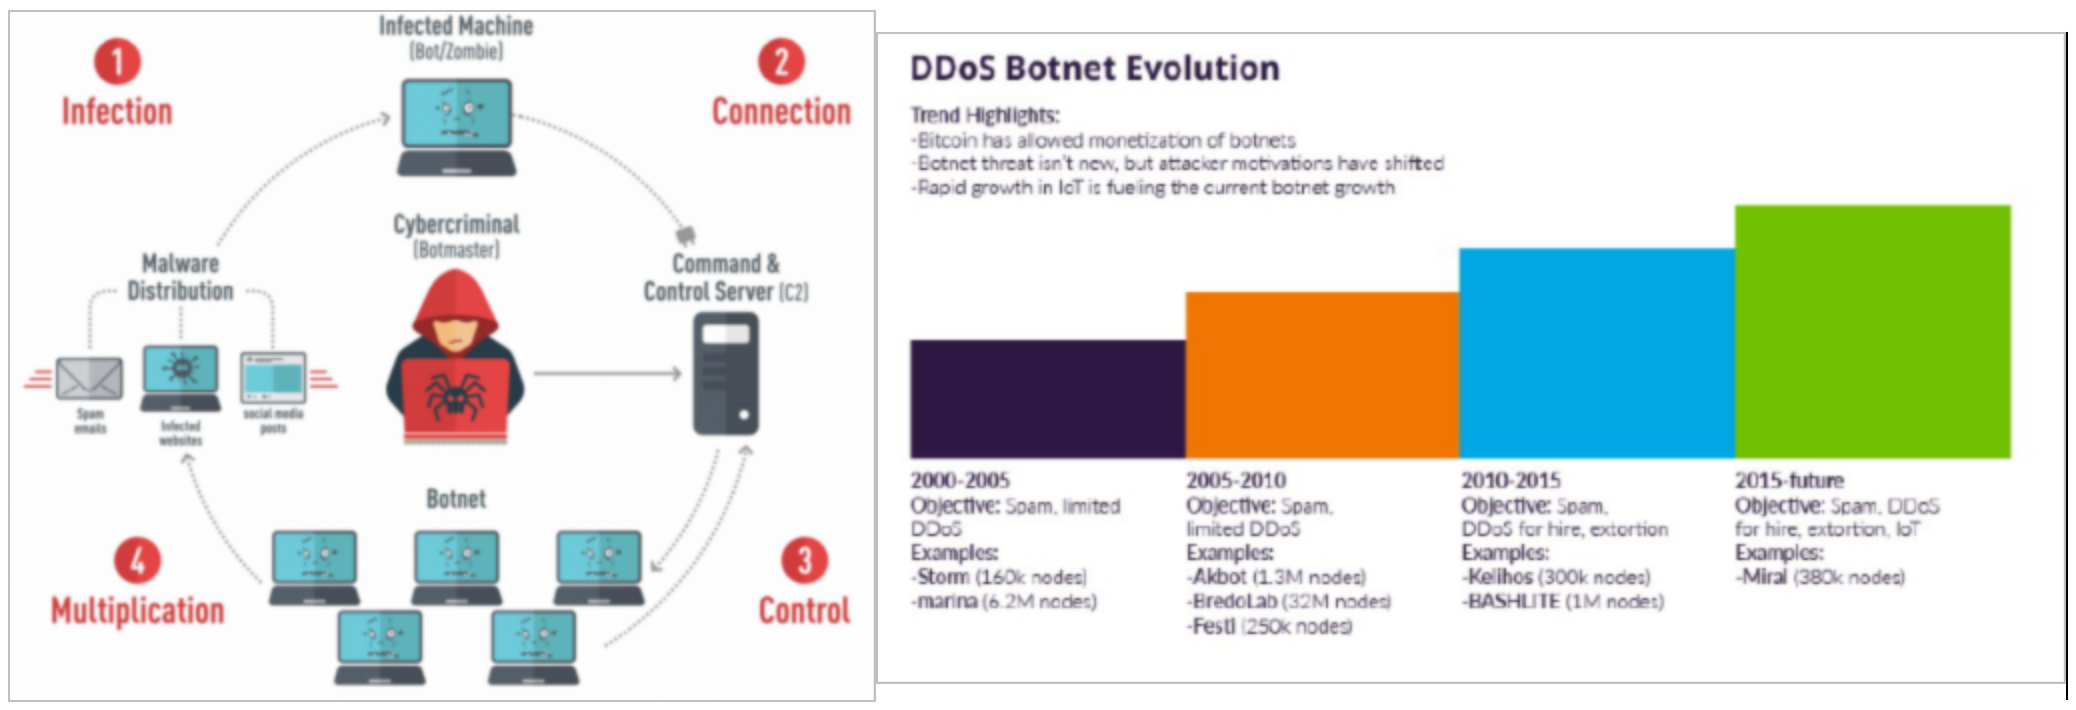
\includegraphics[scale=0.22]{images/DK1.png}
    \caption{Schema ed evoluzione delle Botnet}\label{fig:1}
\end{figure}
Le botnets si sono evolute in modo da amplificare il loro raggio d’azione:
\begin{itemize}
    \item DDoS DNS amplification si basa sulla modifica di un pacchetto, cioè si invia la richiesta di un servizio ad un certo server, 
    ma il pacchetto manomesso non conterrà come sorgente l’indirizzo IP dell’attaccante, bensì quello della vittima. Tutte le risposte 
    verranno dirottate verso l’indirizzo IP della vittima. L’attaccante si avvale di una botnet per effettuare l’attacco. Il meccanismo 
    si basa sull’amplificazione della risposta rispetto alla richiesta, ad esempio una query UDP di 60 byte può generare una risposta 
    di 512 byte (8.5 volte più grande).
    \item Memcached attack l’attaccante dirotta verso una vittima, le risposte alle richieste che vengono effettuate ad un memcached 
    server( server basato su un database di cache per aumentare la velocità di reti e siti web), così andando ad “allagare” tutte le 
    risorse della vittima. Quando anche la rete viene sovraccaricata, le richieste non possono più essere fatte e non è più possibile 
    accedere alle risorse internet, in questo caso ci si trova in una situazione di denial-of-service
\end{itemize}
\textbf{Record di attacco DDoS = 1.7 Tbps} \\
Chiave di sicurezza:
\begin{itemize}
    \item Confidenzialità: Assicura che non vengano divulgati dati sensibili, ma che si possa scegliere cosa deve essere raccolto e/o memorizzato
    \item Integrità dei Dati: Informazioni e programmi possono essere cambiati solamente in una maniera autorizzata e specificata
    \item Integrità di sistema: Assicura che il sistema esegua le sue operazioni in un’unica maniera e che funzioni tempestivamente senza mai 
    negare i servizi agli utenti autorizzati
\end{itemize}
\section{Casi interessanti}
\subsection{Hacking Team}
Hacking Team è una società di Information technology con sede a Milano. Vende servizi di intrusione offensiva e di 
sorveglianza a moltissimi governi, organi di polizia e servizi segreti di tutto il mondo. Da quanto affermato 
dall'hacker nel suo documento, Hacking Team aveva poco esposto su internet. Aveva il suo sito principale 
(in Joomla, senza particolari vulnerabilità), un server di posta, un paio di router e di dispositivi 
Vpn e un dispositivo per filtrare spam. Per cui aveva tre opzioni: trovare uno 0day per Joomla, 
uno per postfix e uno per i sistemi integrati. (Uno 0day è una vulnerabilità di un software ancora sconosciuta, se non all’attaccante). 
L’hacker dice di aver scelto la terza opzione e di aver ricavato un exploit, un codice con cui sfruttare una data 
vulnerabilità, in due settimane. Attraverso questo avrebbe bucato i servizi esposti (router o Vpn) di Hacking Team, 
anche se nella guida dice di non volere dare troppi dettagli perché le vulnerabilità usate 
non sarebbero state ancora messe a posto (patchate). Si sarebbe anche scritto una backdoor per avere persistenza 
e “per proteggere l’exploit” e avrebbe passato settimane a provare exploit, backdoor e altri strumenti sulle 
reti di altre aziende prima di entrare in quella della società milanese. Una volta dentro al network avrebbe 
iniziato un lavoro di espansione, puntando alla posta e scaricandosela, quindi le macchine virtuali, 
infine sarebbe entrato nei pc degli admin, ottenendo sempre più credenziali fino ad arrivare al server 
“Rete sviluppo” dove stava il codice sorgente di Rcs, il software sviluppato da Hacking Team. 
Infine avrebbe preso possesso del profilo Twitter dell’azienda attraverso la funzione “Password dimenticata”.
“Questo sono la bellezza e l’asimmetria dell’hacking: con un centinaio di ore di lavoro una sola persona può disfare 
anni di lavoro di una impresa multimilionaria. L’hacking dà la possibilità agli spossessati di lottare e vincere”.
L’hacker conclude dedicando il suo scritto alle “vittime dell’assalto alla scuola Armando Diaz e a tutti quelli 
che hanno sparso il loro sangue per mano dei fascisti italiani”. Il riferimento è ovviamente al pestaggio 
avvenuto alla scuola di Genova durante il G8 del 2001 da parte delle forze dell’ordine.
\subsection{Carbanak}
\noindent
Dal 2013 in avanti, diverse banche e istituti finanziari hanno subito attacchi da parte di un gruppo 
di cybercriminali che utilizzavano un modus operandi simile. Secondo le vittime e le forze dell’ordine, 
le perdite totali derivanti dagli attacchi ammonterebbero a 1 miliardo di dollari. \\\\
L’analisi degli attacchi ha mostrato che l’infezione iniziale è stato effettuata utilizzando emails di 
phishing che apparivano come comunicazioni bancarie e che avevano un file .doc (realizzato con Word 97-2003) 
e un file .cpl (Control Panel Applet) come allegati.\\\\
I file allegati sfruttavano delle vulnerabilità in Office 2003, 2007 e 2010 (CVE-2012-0158 e CVE-2013-3906) 
e in Word (CVE-2014- 1761). Una volta che le vulnerabilità erano state exploitate con successo, lo 
shellcode decripta ed esegue la backdoor conosciuta come \textbf{Carbanak}.\\\\
Carbanak è una backdoor remota (basata inizialmente su Carberp) pensata per spionaggio, esfiltrazione 
di dati e fornisce un accesso remoto alle macchine infette. Una volta che l’accesso è garantito, gli 
attaccanti eseguono una ricognizione “manuale” della rete della vittima.\\\\
Gli attaccanti hanno utilizzato diversi tools per garantirsi l’accesso ai sistemi critici 
dell’infrastruttura delle vittime. In seguito, gli attaccanti hanno installato del software addizionale, 
come Ammy Remote Administration Tool, oppure hanno compresso i server SSH. Notare che alcune delle ultime 
versioni analizzate di Carbanak non utilizzano alcun sorgente di Carberp.\\\\
Una volta che gli attaccanti hanno compromesso con successo la rete delle vittime, le destinazioni interne 
principali sono i servizi di money processing, gli ATM e i conti finanziari. In alcuni casi, gli attaccanti 
hanno usato la rete SWIFT (Society for Worldwide Interbank Financial Telecommunication) per trasferire il 
denaro sui loro conti. In altri casi, i database Oracle sono stati manipolati per aprire conti con carte 
di pagamento o di credito presso la stessa banca o per trasferire soldi tra i conti utilizzando il sistema 
di banking online. La rete di ATM è stata utilizzando per erogare contanti da determinati ATM in 
determinati orari dove alcune persone (dette money mules) erano pronti a raccoglierli.\\\\
Come parte della fase di ricognizione, sono state realizzate delle registrazioni video delle attività 
degli impiegati delle banche, in particolare dei system administrators. I video sono poi stati mandati 
al server C2.\\\\
Da notare che gli attaccanti hanno abusato dei servizi nominati prima impersonando utenti locali reali 
che avevano il permesso di eseguire le azioni replicate in seguito dagli attaccanti: nessuno dei 
servizi nominati è stato attaccato.\\\\
Delle 100 banche attaccate, almeno la metà hanno sofferto di perdite finanziarie. Molte vittime, 
basandosi sul loro IP, si trovano in Russia, USA, Germania, Cina e Ucraina.\\\\
I fondi rubati sono stati trasferiti fuori dalle nazioni infettate in conti bancari in USA e Cina. 
Alcuni log dei server C2 mostrano connessioni con sistemi localizzati negli USA. La telemetria 
indica che gli attaccanti stanno espandendo le loro operazioni in altre regioni, come Asia, 
Middle-East, Africa ed Europa. 

\subsection{APT32 / OceanLotus}
\noindent
APT32 o OceanLotus sono un gruppo di hacker che hanno portato avanti intrusioni in compagnie private 
e hanno preso di mira governi stranieri, dissidenti e giornalisti. FireEye (esperti di sicurezza) 
sostiene che APT32 hanno rilasciato una suite unica di malware completi, in unione con tools commerciali, 
per condurre operazioni mirate allineate con gli interessi dello stato del Vietnam. \\\\
Passiamo ora all’analisi del file: la prima cosa che si nota è che il file binario/exe utilizza 
l’icona di un file .doc per farsi passare come un documento di Word: questo per indurre l’utente a 
credere che il file sia un comune documento Word (quindi un file che non nasconde alcun pericolo). \\\\
Alcuni siti che vengono spesso utilizzati per condurre un’analisi approfondita su un file e cercare 
quindi di raccogliere il maggior numero possibile di informazioni è app.any.run, Hybrid Analysis e 
VirusTotal. Dopo una piccola ricerca si inizia dunque l’analisi comportamentale del file per cercare 
di replicare i risultati dei siti e per scoprire eventualmente nuove caratteristiche descritte 
riscontrate sul file.\\\\
Per prima sono stati settati fakedns, inetsim e Wireshark per emulare servizi Internet. Bisogna 
poi assicurarsi che la VM che si sta utilizzando si trovi in un ambiente il più isolato possibile, 
in modo da poter mitigare eventuali danni. Se il campione (il file analizzato) richiede l’accesso 
a Internet (e quindi “esce” dalla VM), bisogna assicurarsi di essere in una rete isolata.\\\\
Il file cerca di connettersi, attraverso Internet, al dominio che si trova nel campo “Referer”. 
La connessione viene creata da uno dei file scaricati (rastlsc.exe): questo tenterà di stabilire 
una connessione verso l’esterno e successivamente killerà sé stesso. 
\begin{figure}[H]
    \center
    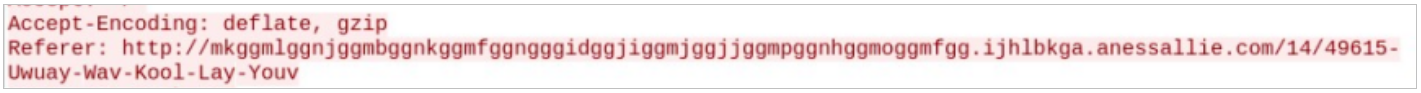
\includegraphics[scale=0.25]{images/OceanLotus1.png}
    \caption{Campo “Referer”}\label{fig:1}
\end{figure}
\noindent
Il campione cercherà anche di connettersi a numerosi registri associati alla suite Office.\\\\
In seguito, verrà creato un file tmp.docx: questo file, insieme a rastlsc.exe, 
sono creati con l’API di Windows CreateFileW.\\\\
Il compito principale di questo file sembra quindi quello di scaricare altri files (dropper), 
preparare l’ambiente e creare una connessione verso l’esterno con rastlsc.exe.
\begin{figure}[H]
    \center
    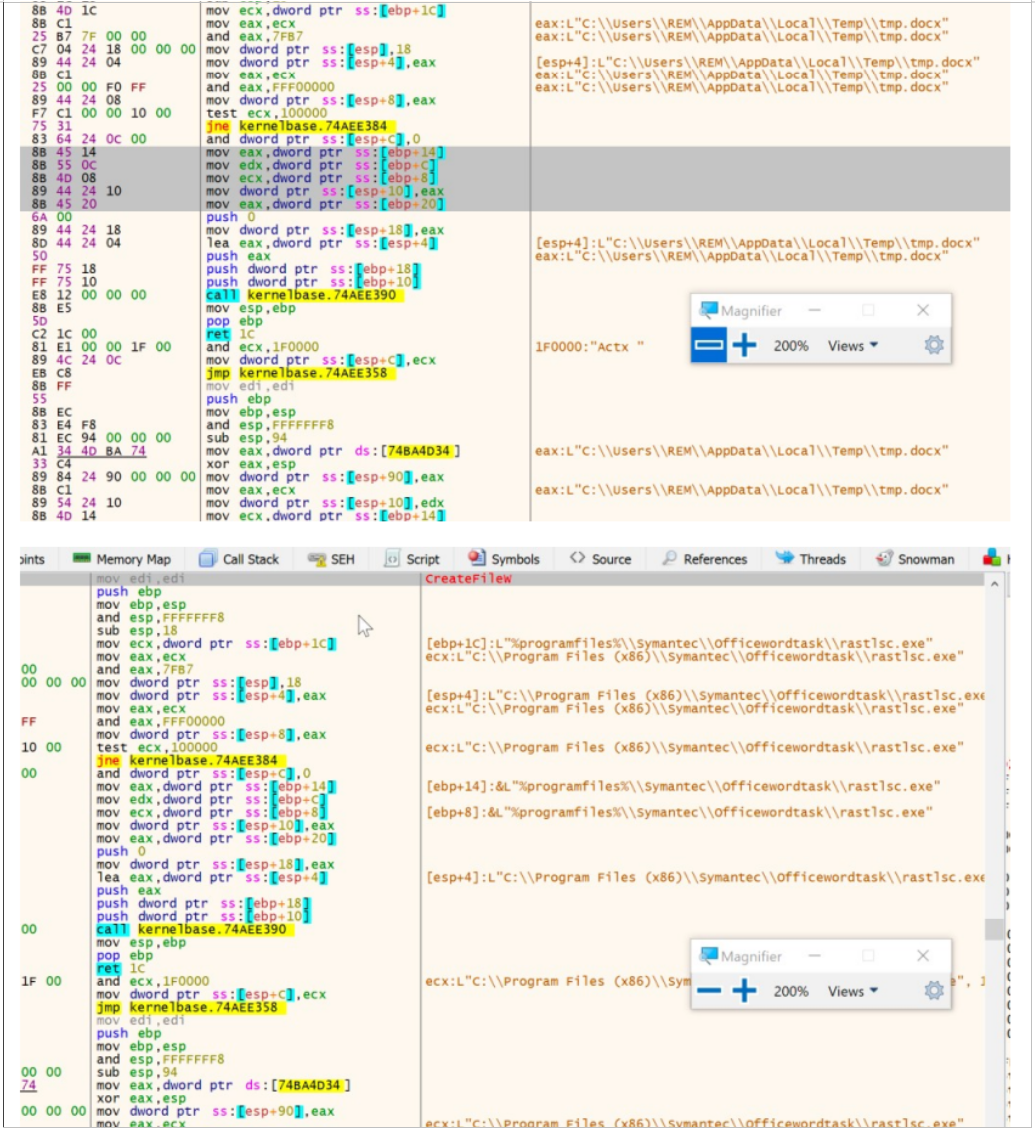
\includegraphics[scale=0.3]{images/OceanLotus2.png}
    \caption{Reverse code}\label{fig:1}
\end{figure}
\subsection{Wannacry}
WannaCry è un ransomware (un cryptoworm, per essere ancora più specifici), cioè un particolare tipo di malware che 
rende inaccessibili i dati dei nostri computer e, per ripristinarli, chiede un riscatto da pagare in bitcoin, 
la moneta elettronica. Il malware colpisce chi ha il proprio computer collegato alla Rete e ha un sistema operativo 
Windows, dato che il software malevolo si propaga grazie a EternalBlue, un codice della Nsa (l’agenzia per la 
sicurezza nazionale statunitense), pubblicato online lo scorso aprile dal gruppo hacker Shadow Brokers. 
Uno strumento che sfrutta la vulnerabilità di un protocollo di condivisione di file di rete, SMB (Server Message Block), 
usato da sistemi Microsoft Windows.\\\\
Ma come avviene la prima infezione? Inizialmente, si pensava che il vettore d’attacco originario fosse la posta 
elettronica. Successivamente, però, la tesi più accreditata è che il malware si diffonda “attraverso computer 
vulnerabili esposti su internet con la porta 445. Una volta che un solo computer di una rete locale viene infettato, 
il malware automaticamente si propaga usando il protocollo SMB”, come si legge nelle raccomandazioni del Cert-EU, 
l’unità europea per la risposta alle emergenze informatiche, che aggiunge: “è importante menzionare che computer 
non aggiornati e reti esposte via SMB su internet possono essere infettati direttamente senza il bisogno di altri 
meccanismi. Basta che siano accesi e accettino connessioni SMB”.\\\\
La peculiarità originale di WannaCry, rispetto ad altri ransomware più “classici” è che si tratta di un malware 
costituito da due componenti che operano in successione:
\begin{enumerate}
    \item Un exploit (trattasi di malware realizzati appositamente per sfruttare una “falla” di un sistema) 
    che sfrutta la vulnerabilità SMBv1 per attaccare il computer obbiettivo.
    \item Un ransomware vero e proprio che esegue la cifratura dei files.
\end{enumerate}
Secondo Microsoft gli scenari presunti d’attacco sono due (Microsoft parla di scenari “altamente probabili”, 
senza indicarli come assolutamente certi):
\begin{enumerate}
    \item Tramite le solite email di phishing (contenenti finte fatture, note di credito, bollette, ecc.), 
    o tramite chiavette USB (come successo all’Università Bicocca). Questi sono i vettori d’attacco tipici e 
    più frequenti per la maggior parte dei ransomware.
    \item Tramite attacco diretto mediante Exploit attraverso il protocollo SMB in macchine non aggiornate.
\end{enumerate}
Quindi, importante esserne consapevoli, se il sistema è affetto dalla citata vulnerabilità, non serve 
necessariamente l’email di phishing per subire l’attacco. In parole più semplici e banalizzando il concetto: 
non occorre che siamo noi ad aprire la porta, perché è l’hacker a possedere già la chiave (cioè l’exploit). 
Una volta entrato in un computer (ne basta uno solo!) di un sistema Windows, WannaCrypt si propaga in modo 
automatico agli altri computer (anche se non collegati ad Internet) sfruttando le condivisioni di rete SMB, 
attraverso le porte di comunicazione 139 e 445. Questo spiega la rapidità (insolita) con cui si è diffuso.\\\\
Poi – secondo passaggio – esegue una criptazione dei files, usando una crittografia RSA a 2048 bit (quindi 
assolutamente inattaccabile).\\\\
I files crittografati vengono rinominati aggiungendo l’estensione .WNCRY, quindi, per esempio, un file 
picture.jpg verrà modificato in picture.jpg.WNCRY.\\\\
WannaCry provvede inoltre ad eliminare le “Shadows copies” di Windows (per impedirci di recuperare i dati) 
e va a scrivere in alcune tipiche cartelle di sistema, quali:
\begin{itemize}
    \item \%SystemRoot\%
    \item \%SystemDrive\%
    \item \%ProgramData\%
\end{itemize}
Altra peculiarità: a causa del tipo di vulnerabilità, il malware riesce ad installarsi anche se l’utente non 
ha diritti di amministratore, ma è un semplice utente.
\end{document}